\chapter{Object~Detection}
\label{chap:object_detection} 

\section{Introduction}

In this chapter I describe the object detector, training and evaluation metrics used in the object detection annotation system described in chapter~\ref{chap:design} and used in this thesis. I describe the object detector, and describe the key differences and the motivations behind those differences in adapting this object detector for the purposes of assisting annotation.

The object detector is based off a single-shot \gls{CNN} detector called RetinaNet \cite{Lin2017}, which was selected for it's simplicity and efficiency, while having close to state of the art accuracy. The major differences from the method in \cite{Lin2017} and brief motivations for each are:

\begin{itemize}
    \item Shared weights between classification sub-networks at different pyramid levels. This was found to make training much faster at the beginning.
    \item No normalisation of the loss function (by number of anchor matches), in order to accommodate images with no positive annotations.
    \item Training on crops of very high resolution images, but evaluation on complete images.
    \item Use of cyclical learning rates in training, to accommodate incremental additions to the training set.
\end{itemize}

Each described in more detail later in this chapter. After describing the details of the object detector we test some of the hypotheses which led us to these decisions (amongst others) in section~\ref{sec:experimental_validation}.

\section {Image preparation}

One thing which was noticed in the implementation of the segmentation tool from chapter~\ref{chap:bootstrap} was that the original images were often much clearer than the scaled down images for a human annotator to see fine details which can be lost at lower resolution. 

High resolution images present a cost in terms of training (and inference) time, also in terms of memory and data required to transfer over a network. High resolution images are undoubtedly easier to annotate, small details become clear and using down scaled images often makes even the annotation task ambiguous. It is not necessary to feed the model images of the same resolution as the user annotates, but if a human annotator has trouble with ambiguity it seems a reasonable assumption that a \gls{CNN} will also struggle, especially for datasets with many small examples. The datasets used here (see chapter for details~\ref{chap:datasets}) contain many small objects, and many objects with a high degree of uncertainty and ambiguity.

With that in mind I focused on preserving resolution for the annotation process. High resolution images present a cost in terms of training (and inference) time, also in terms of memory and data storage and data transfer over a network, all of which make smaller images preferable. In section~\ref{sec:scale_crop} I experimentally validate this idea, comparing training with different resolutions (and crop sizes) for a selection of datasets.

In object detection datasets, larger objects have consistently been shown to have a higher accuracy than medium or small objects \cite{Lin2014, Wang2017, Lin2017a, Law2018, Zhou2019}. In the COCO dataset, small being defined as having an area of $<32^2$ and large having an area of $>96^2$ pixels. In addition detectors trained at higher resolutions on the same datasets consistently show higher performance.

 Compared to the PASCAL VOC \cite{Everingham2008}, or COCO \cite{Lin2014} datasets which have a large range of scales; the majority of data experimented on in this thesis, the objects of interest occupy an area much smaller than the whole image size. An analysis of object sizes of two of the less extreme datasets compared to VOC and COCO can be seen in figure~\ref{fig:box_sizes}. 

We hypothesise that it is possible to get away with larger image sizes by using smaller crops of the original images to train, as long as the objects fit in the image crops. We do some experiments on this idea in section~\ref{sec:validation}, in order to test this hypothesis. When trained at a full resolution, the number of objects considered to be large by the COCO definition is greatly increased.

Use of simpler, faster models has been successful as the backbone of the object detection network (for example ResNet--18), which enables larger images in both training and evaluation. Time taken for evaluation and training is also much improved relative to using larger networks. For the smaller datasets in our experiments I did not see large improvements in accuracy when using larger backbone networks.

\begin{table}[h]
  \centering
    \caption{Ranges of parameters used for image augmentation, translation occurs as part of a cropping process}
    
  \begin{tabular}{ l  l }
    Parameter & Range \\
    \toprule
    scale (log uniform) & ${3/4}$--${4/3}$  \\ 
    aspect scale  & $ 1 \pm 0.1 $  \\ 

    brightness adjustment (additive) & $ \pm 10 $ \\ 
    contrast (multiplicative) & $ 1 \pm 0.1 $ \\ 

    gamma adjustment & $ \pm 0.1 $ \\ 

    hue shift & $ \pm 5 $ \\ 
    saturation shift & $ \pm 5 $ \\ 
    
    horizontal flips & $ P = 0.5 $ \\ 
    
    \bottomrule
  \end{tabular}
\label{fig:obj_augmentation}
\end{table}

After applying augmentation (photo-metric distortion and scaling) with parameters described in table~\ref{fig:obj_augmentation} and image whitening (described below), a region is cropped from the resulting image at random. In the case where the crop region is larger than the input image, an image is created with pixels set to zero and the input image is placed at a random position within the image.

The crop sizes used in experiments, and in image annotation are specific to each dataset, ranging from $1024\times1024$ for the \emph{apples1} and \emph{apples2} datasets, down to $320\times320$ for the \emph{branches} dataset.

We employ image whitening to ensure consistency with ImageNet trained models (used as the backbone of the networks) subtracting mean (r, g, b) $ (0.485. 0.456, 0.406) $ and dividing by standard deviation $ (0.229, 0.224, 0.225) $.


\section {Object detection}

The object detection method I have been using for the following experiments is a modified RetinaNet \cite{Lin2017} as a strong near-state of the art object detector with a simple implementation. RetinaNet is a type of single shot object detector, meaning that it detects all objects together in one pass, as opposed to two stage detectors which first identify sets of bounding box proposals and then have a second pass to refine those box proposals into concrete detections. Single shot detectors (such as \gls{SSD} \cite{Liu2016a} or RetinaNet) typically achieve faster inference and training time by skipping the second refinement phase, at a slight cost of accuracy.  

Many object detection methods are based on sliding windows, where windows of fixed sizes are moved across an image and attempt to match objects of that size at each position. \gls{CNN} based object detectors achieve this using anchor boxes, where the sliding window is replaced by a simultaneous matching of boxes at each point across an image. Using a fixed set of anchor boxes limits the localisation accuracy, so the counter point to matching anchor boxes is also estimating a transformation to refine an anchor box to fit the more specific size of the object.

RetinaNet is based off Feature Pyramid Networks \cite{Lin2017a} which uses feature maps produced at multiple levels of a \gls{CNN} to classify anchor boxes of different sizes, where many smaller anchor boxes match smaller objects on higher resolution feature maps and fewer larger anchor boxes match larger objects. 

The object detection models bear close similarly to the segmentation models discussed and used in chapter~\ref{chap:bootstrap}, such as UNet \cite{Ronneberger2015}. \gls{FPN} models utilise shortcut connections in the same way, the major difference from segmentation models is that anchor boxes are predicted at multiple levels, where segmentation models output mask predictions only at one resolution.


\subsection {Network architecture}
\label{sec:architecture}

Some parameters and network architectures differ from \gls{FPN} \cite{Lin2017a}. For the most part the modifications are small things which seem to enable it to learn better on the kind of small datasets used for experiments in this work. These include adding extra residual layers to the decoder, shown in figure~\ref{fig:detection_network}. It is more similar to the network shown in ~\ref{chap:bootstrap} than the \gls{FCN} network. A key difference is that neither the weights between classification sub-networks nor box regression subnets are shared between different scales  (the original shares weights between classification sub-networks). I found in the small scale datasets used in this work that shared weights on the class sub-network significantly slows initial learning. The extra residual layers in the decoder side of the network (figure~\ref{fig:decoder_block}) improved this significantly, but not entirely. 

\begin{figure}[h]
  \centering
  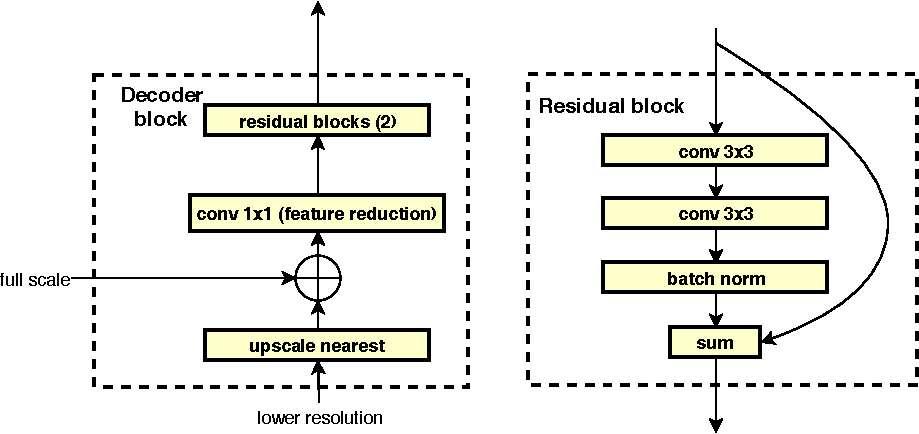
\includegraphics[width=1.0\linewidth]{figures/annotation/decoder_block.pdf}
  \caption{Decoder block, responsible for merging half resolution features with features from full resolution skip connections }  
  \label{fig:decoder_block}
\end{figure}


\begin{figure}[h]
  \centering
  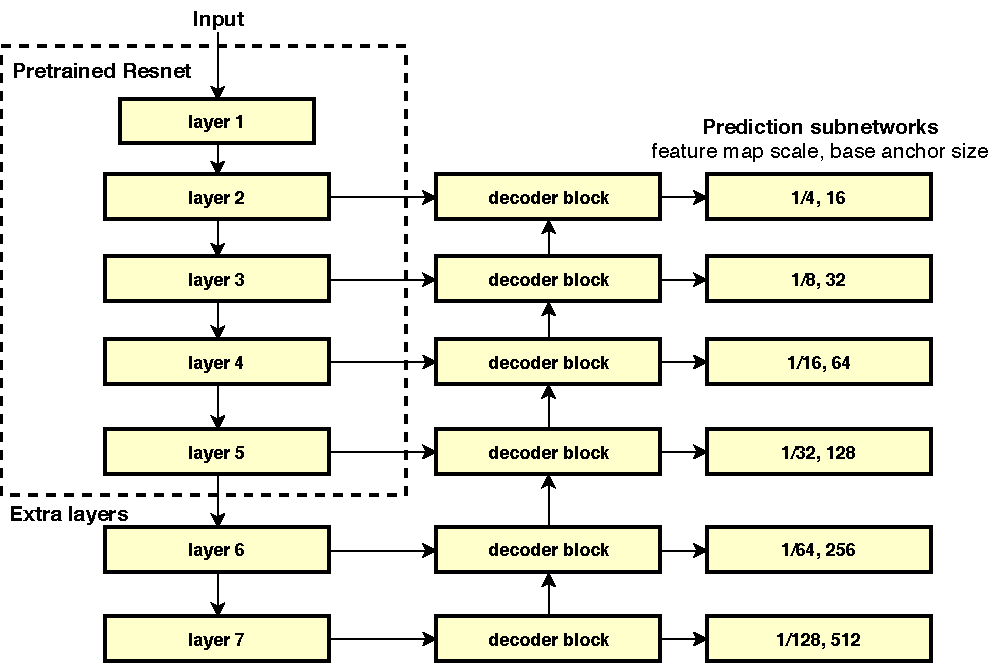
\includegraphics[width=1.0\linewidth]{figures/annotation/detection_network.pdf}
  \caption{Object detection network, built on the backbone ResNet }  
  \label{fig:detection_network}
\end{figure}

\begin{figure}
  \centering
  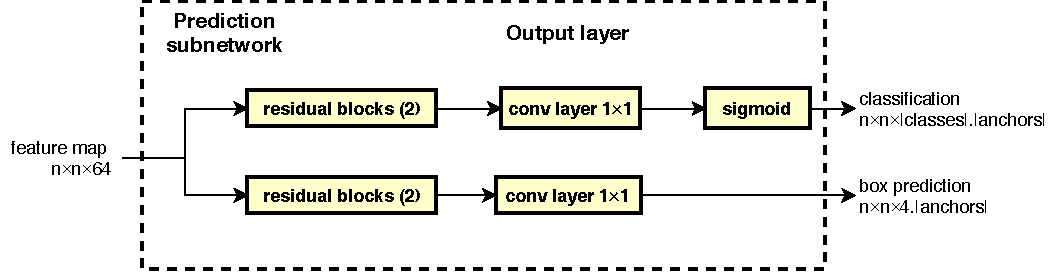
\includegraphics[width=1.0\linewidth]{figures/annotation/prediction_subnet.pdf}
  \caption{Prediction sub-network with two streams, one for classifying anchor boxes with one output per class for each anchor box, the other stream for location regression for each anchor box (shared between classes)}    
  \label{fig:prediction_subnet}  
\end{figure}

\subsection{Initialisation}

The initialisation used is as in \cite{Lin2017}; where all new convolutions added to the backbone are initialised with $\sigma=0.1$ (and no bias). The final layer of the classification sub-network has bias initialised to $b = −log((1 − \pi)/\pi) $ whereby at the start of training every anchor box is assigned confidence of $~\pi$, we use $\pi=0.01$. With this initialisation training becomes robust to a wide range of resolutions and learning rates.

\subsection{Anchor boxes}

\begin{figure}
  \centering
  \begin{subfigure}[t]{0.33\textwidth}
  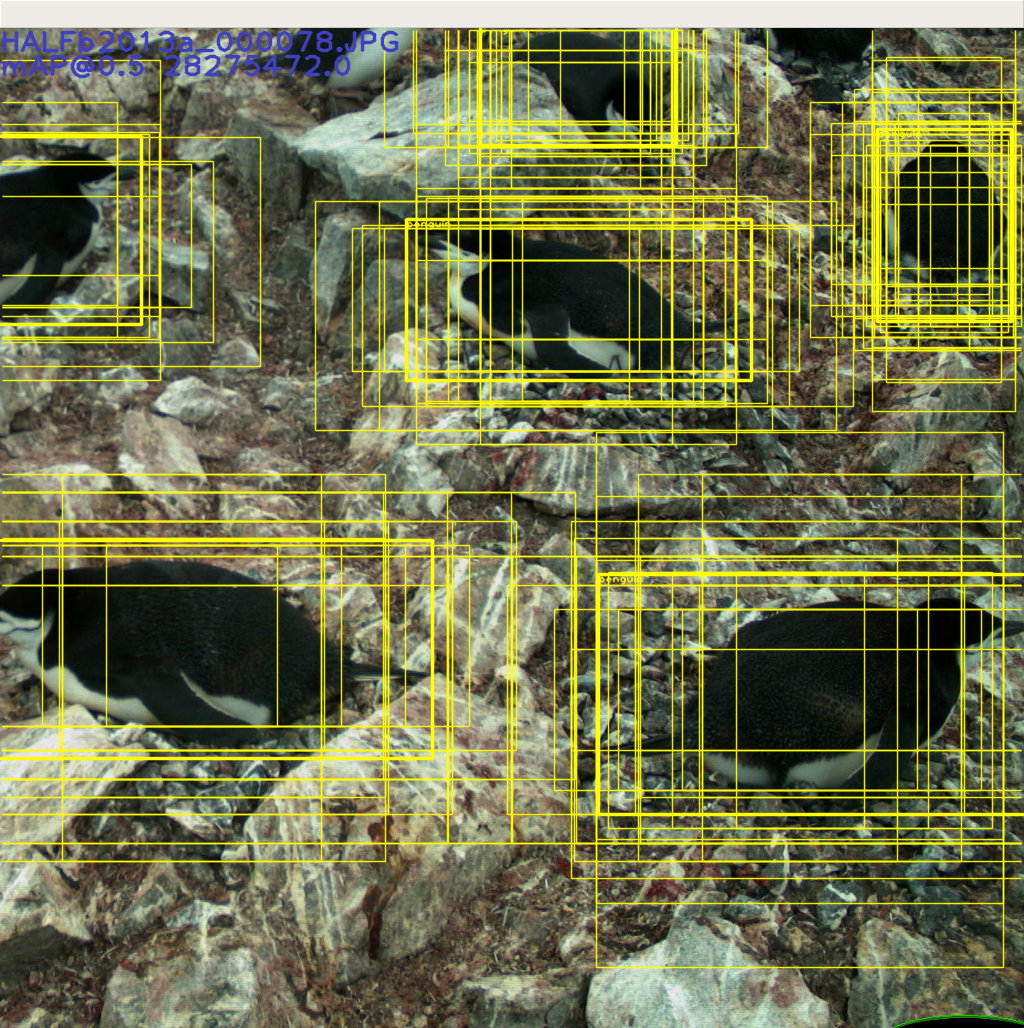
\includegraphics[width=0.95\linewidth]{figures/object/anchors.png}
  \caption{Anchor boxes from class predictions}
  \end{subfigure}%
  \begin{subfigure}[t]{0.33\textwidth}
  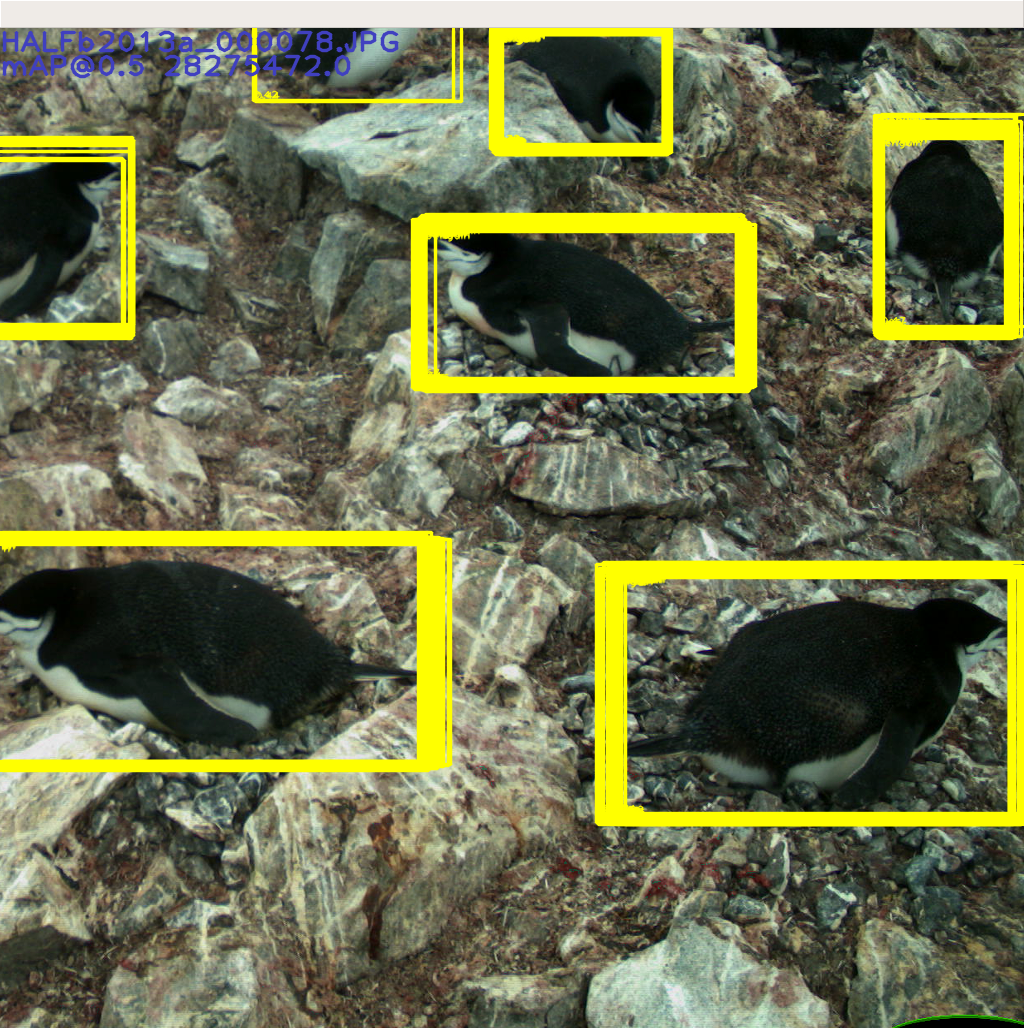
\includegraphics[width=0.95\linewidth]{figures/object/predictions.png}
  \caption{Refined anchor boxes after transformation}
  \end{subfigure}%
  \begin{subfigure}[t]{0.35\textwidth}
  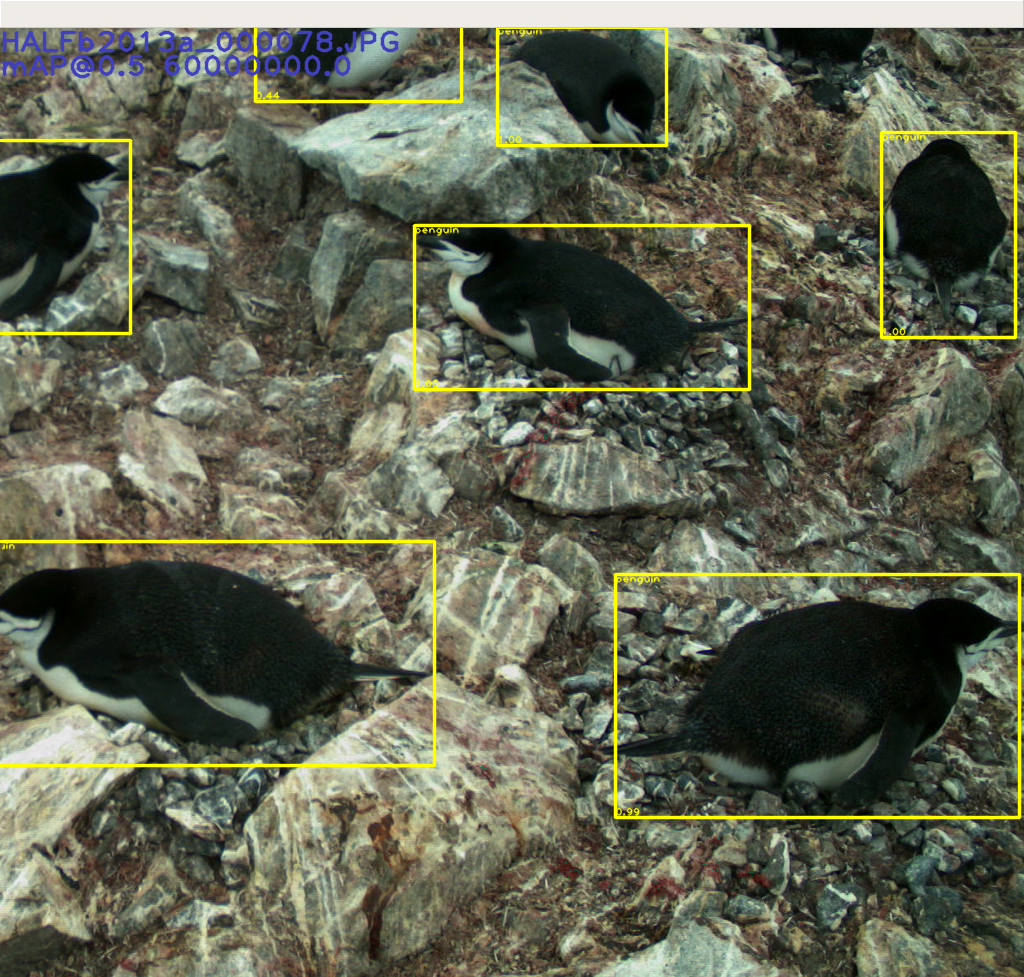
\includegraphics[width=0.95\linewidth]{figures/object/final.png}
  \caption{Final predictions after Non Maxima Suppression}
  \end{subfigure}%  
  \caption{Illustration of the stages of box prediction and refinement process}
  \label{fig:anchor_boxes}
\end{figure}


We use translation invariant anchor boxes as per \cite{Wang2017}, anchor boxes are the set of default locations and box sizes for which the \gls{CNN} can predict if and which object exists. It is unfeasible to provide a discrete set of boxes large enough to cover all possible object locations, therefore each anchor box is also modified by a scale and translation (details below in section~\ref{sec:regression}) to fine tune anchor boxes to fit objects in the image.

Set of anchors boxes are used for each level with aspect ratios $ \in \{0.5, 1, 2\} $ and scales $ \in \{2^0, 2^{1/3}, 2^{2/3}\} $. For each feature map at level $k$, with a base scale of $ 2^{k + 2} $ pixels, the set of 9 anchor boxes (all combinations of aspect and scale) are tiled centred on each feature map pixel. 

In the case of counting, where circles are used for annotation only three anchor boxes are used, only the square aspect ratio is used at the same three scales. For all intents and purposes the circles with radius $r$ are treated as a square box with side lengths $2r$, and the box regression sub-network modified to produce only $3$ outputs (enforcing square aspect ratio for height and width).

Feature maps on levels $3$--$7$ are used for most datasets giving the smallest (square) anchor at $32\times32$ and the largest at $812\times812$. In the case of datasets with very small objects (for example, aerial penguin counting and wide angle counting of seals) we add in anchor boxes on level 2 which allow for objects as small as $16 \times 16$.

For those with smaller objects such as the aerial Adellie penguin counting, the tree branch detection and the seal counting an extra feature map is used giving anchor boxes as small as $16\times16$ and more densely tiled.

In training, anchor boxes are selected by matching on \gls{IOU} overlap with ground truth boxes. Each anchor is matched with the ground truth box with highest overlap. An anchor box matches a ground truth box as a positive if $ IoU >= 0.5 $, anchors with $ IoU < 0.4 $ are treated as negative, and those boxes with $ 0.5 > IoU >= 0.4 $ are ignored (omitted from either positive or negative for computing loss).

Ground truth boxes will match with potentially many anchor boxes, but those in close proximity and similar size may mean that boxes which would have otherwise matched do not, because anchors cannot be assigned to more than one ground truth.

\subsection{Total loss function}

The total loss function is defined as a balanced sum between box regression ($L_{loc}$) and class prediction loss ($L_{class}$). 

\begin{equation}
L  = L_{loc} + \lambda L_{class}
\label{eq:loss_total}
\end{equation}

\subsection {Box regression loss}
\label{sec:regression}


We use the anchor box encoding used in \gls{RCNN} \cite{Wang2017} for the purpose of calculating location loss. The loss is a smooth-L1 loss over regression target ($t^*_x, t^*_y, t^*_w, t^*_h \in t^*_i$) giving a transformation from an anchor box ($a_x, a_y, a_w, a_h$)  to a set of regression targets $t^*_i$ from the ground truth ($g_x, g_y, g_w, g_h$). 

The boxes are encoded as the offset of the centre in both directions (in proportion to the box size) and the log scale of height and width. The encoding of the four targets are given as:

\begin{equation}
\begin{split}
t^*_x = (g_x - a_x) a_w\\
t^*_y = (g_y - a_y) a_h\\
t^*_w = log(g_w / a_w)\\
t^*_h = log(g_h / a_h)\\
\end{split}
\label{eq:encoding_rcnn}
\end{equation}

The localisation loss can be directly computed from these targets and the output of the box prediction sub-network as the sum smooth-L1 regression of $t_i^* - t_i$. Smooth-L1 is a combination of L2 loss near the origin and L1 loss otherwise. It is given as:

\begin{equation}
L_{1;smooth} = 
\begin{cases*}
|x| & if $|x|>\alpha $ \\
\frac{1}{|\alpha|}x^2 & if $|x| \leq \alpha$
\end{cases*}
\label{eq:smooth_l1}
\end{equation}

The commonly used value $\alpha = 0.5$ is used here. The total localisation loss is then summed across matching (\gls{IOU} > 0.5) anchor truth boxes as:

\begin{equation}
L_{loc} = \sum_i{L_{1;smooth}(t_i^* - t_i)}
\label{eq:loss_loc}
\end{equation}

By rearranging the equations we can then do the reverse process and decode bounding boxes from box predictions $t_x, t_y, t_w, t_h$  and an anchor box. These predictions are then in units of pixels and given as the predictions of the object detection network (after a \gls{NMS} process to cull duplicates).

\begin{equation}
\begin{split}
p_x = a_x + t_x  a_w\\
p_y = a_y + t_y  a_h\\
p_w = exp(t_w) a_w \\
p_h = exp(t_h) a_h\\
\end{split}
\label{eq:decoding_rcnn}
\end{equation}

\subsection {Classification loss}
\label{sec:loss}

The experiments use a modified version of the Focal Loss \cite{Lin2017} to handle the class imbalance (negative vs. positive) present when sampling anchor box predictions densely.

Focal Loss \cite{Lin2017} re-weights the standard \gls{BCE} loss function to deal with a large number of easy negative examples in object detection (the number of unmatched anchor boxes greatly outnumbers the number of matched anchor boxes). Focal Loss enables dense sampling of negative examples present in an image. The standard approach in to dealing with the imbalance between positive and negative examples has been to sample the most significant negative examples to provide a certain positive to negative ratio.

As defined \cite{Lin2017}, we use the same terminology and variable naming for consistency. The basic two class \gls{CE} equation for binary prediction from the model classifier $p \in \left[0, 1\right]$, and label $y \in \{0, 1\}$  is given:

\begin{equation}
CE(p, y) = 
  \begin{cases*}
  -log(p) & if $y = 1$\\
  -log(1-p) & otherwise\\
  \end{cases*}
\label{eq:cross_entropy}
\end{equation}


The cross entropy can be rewritten by defining $p_t$ the prediction relative to the given label.

\begin{equation}
p_t = 
  \begin{cases*}
  p & if $y = 1$\\
  1 - p & otherwise\\
  \end{cases*}
\label{eq:class_prob}
\end{equation}

Allowing the \gls{CE} equation to be rewritten more simply:

\begin{equation}
CE(p_t) = -log(p_t)
\label{eq:short_cross_entropy}
\end{equation}


In order to deal with class imbalance the key idea of \cite{Lin2017} was to re-weight the classification loss to be smaller for well classified boxes (small $p_t$) and to be relatively much larger for badly classified boxes (large $p_t$). This was achieved by multiplying the cross entropy by a factor of $(1 - p_t)^\gamma $ with parameter $\gamma$ a sharpening parameter, to give the focal loss:

\begin{equation}
FL(p_t) = - (1 - p_t)^\gamma log(p_t)
\label{eq:focal_loss_p}
\end{equation}

Another way of dealing with class imbalance is to weight one of the classes. A balanced cross entropy loss can then be written by adding a class weighting $\alpha \in \left[0, 1\right]$ the weight for the positive (rare) case in the two class setting, and an analogous $\alpha_t$:

\begin{equation}
\alpha_t = 
  \begin{cases*}
  \alpha & if $y = 1$\\
  1 - \alpha & otherwise\\
  \end{cases*}
\label{eq:balanced_weight}
\end{equation}

Then the balanced, focused, cross entropy is defined:

\begin{equation}
FL(p_t) = -\alpha_t (1 - p_t)^\gamma log(p_t)
\label{eq:focal_loss}
\end{equation}

I adopt the parameters given in \cite{Lin2017}, using $ \gamma = 2 $, and $ \alpha = 0.25 $. 

The total class loss is then given as the sum of the focal loss computed densely across all classes and anchor boxes in the image (except for anchor boxes between positive threshold and negative threshold $0.4 <= IoU < 0.5$ which are ignored). For $K$ classes, $p_i$ is the size $K$ prediction vector from the network for anchor box $i$ and $p^*_i$ is the size $K$ one hot target vector.

\begin{equation}
\begin{split}
L_{class} = \sum_i{\sum_{k \in K}FL(p_{ik}, p^*_{ik})}
\end{split}
\label{eq:class_loss}
\end{equation}

\subsection {Learning rate and Normalisation}

In \cite{Lin2017} a normalisation occurs over the total loss by the total number of positive matching anchor boxes, in order to average the error from the positive targets (making an assumption that the negative targets contribute a negligible amount to the total loss). As the datasets used in this work often don't contain any positive ground truth boxes it was necessary to avoid a division by zero. One method is to add a constant (representing the contribution of the negative classification targets) to the normalisation factor, the other is to divide by a constant value (essentially using a lower learning rate). I experimented a little with both options, finding either to be reasonably robust, the experiments in this work use a non normalised class classification loss.

In all experiments in this work (unless specified otherwise), the learning rate is set to $0.001$ and the balance factor $\lambda=2.5$. Total loss is averaged across each mini-batch, and batch sizes of $8$ are used.

\subsection{Inference and Non-maxima suppression}

In training a large set of anchor boxes are trained to classify each object detection (those overlapping each anchor box by $0.5$ or more). For the purposes of inference detecting more than one box for the same object is undesirable, so a greedy \gls{NMS} is used to eliminate multiple detections of the same object. Figure~\ref{fig:anchor_boxes} shows the effect of applying a \gls{NMS} on box predictions, (b) shows the regressed predictions where many boxes overlap the same object (c) shows the result of the \gls{NMS}, leaving a single box on each object. In this work a standard \gls{NMS} procedure as per \cite{Wang2017} is used, where boxes are selected from most-confident to least-confident, boxes overlapping lower confidence boxes by more than an \gls{IOU} threshold (in this work $0.5$) are eliminated.

The use of \gls{NMS} has presents some problems in object detectors notably the inability to handle highly overlapping objects well. Objects high overlap by more than $0.5$ are impossible to accurately detect for such a detector. When used for annotating crowded objects the inability of the object detector to accurately predict highly overlapping objects means in some datasets the user spends a lot of time correcting artefacts caused by limitation of the object detector (by no means limited to \gls{NMS}).


\section{Evaluation metrics}
\label{sec:evaluation_metrics}

The most common metric used in object detection is that of \gls{AP}, as popularised by the Pascal VOC challenge \cite{Everingham2008} and later the COCO dataset \cite{Lin2014}. The \gls{AP} is essentially the area under a recall-precision graph for a particular matching threshold and varies from $0$  to $1$. it's major attraction is that it avoids the need for a detection threshold. It provides a single relatively easy to understand metric which measures precision, recall as well as localisation accuracy (for a particular threshold).

Matches are found by a greedy algorithm in each image (similar to that used in \gls{NMS} above) where the predictions are matched against ground truth boxes from a most-confident to lead-confident order. Each prediction matches it's highest overlap ground truth box where the overlap exceeds the \gls{IOU} threshold (amongst ground truth boxes already unmatched). Matches from all images are then merged and sorted by confidence level of the prediction of the match. True-positives ($tp$) and false-positives ($fp$) are found by counting matched and unmatched predictions from high-to-low confidence, false-negatives ($fn$) are determined at each point by subtracting true-positives from the total ground truth count. 

\begin{equation*}
\begin{split}
p_i = \frac{tp_i}{fp_i + tp_i}\\
r_i = \frac{tp_i}{tp_i + fn_i}
\end{split}
\end{equation*}

From there recall ($r$), and precision ($p$) levels can be determined at the confidence level of each prediction. Special cases are added for $r_0=0, p_0=1$ and $p_n=1, r_n=0$, the precision levels are then made monotonic decreasing:

\begin{equation}
\hat{p_i} = \max_{j \in [i..n]}{p_j}
\end{equation}

\gls{AP} can then be calculated by using trapezoid summation:

\begin{equation}
AP = \sum_{i \in [0..n-1]}\frac{\hat{p_i} + \hat{p}_{i + 1}}{2}
\end{equation}


For multiple class object detection the metric is usually the \gls{mAP}, defined as the mean of \gls{AP} across classes. This has the effect of making classes have uniform weight, in the case of an imbalanced dataset.  In this work, I use the simpler overall \gls{AP} instead of the \gls{mAP}, however only a couple of datasets utilise more than one class so in most cases this would be equivalent. To denote the matching threshold used to produce an \gls{AP} we use the notation $AP_{IoU}$ or $mAP_{IoU}$. The most permissive matching threshold used is $0.5$ (used as the primary metric for Pascal VOC), a more strict matching threshold of $0.75$ is often used to measure object detection with strong localisation.

To produce a single metric taking into account localisation accuracy \cite{Lin2014} defined a metric COCO \gls{AP} as the mean of \gls{mAP} at a series of matching thresholds $ IoU \in [0.5 : 0.05 : 0.95] $, confusingly this mean-\gls{mAP} is termed just \gls{AP}. In this work I refer to $AP_{COCO}$ as the average of the $AP_{IoU}$ across this range (instead of the $mAP$) as is usual in the multi-class setting.

\begin{equation}
AP_{COCO} = \frac{1}{10}\sum_{i \in [0.5 : 0.05 : 0.95]}AP_{i}
\label{eq:ap_coco}
\end{equation}

There are downsides to the \gls{AP} family of metrics. The precision-recall graph created using decreasing confidence considers only the order of detection confidence. This has implications that the level of false positives which occur at lower confidence than the last true-positive are ignored, in addition the margin between confidence levels is ignored, so the sensitivity to change in confidence levels is not taken into account. The threshold on \gls{IOU} overlap also means that all true-positives which meet the localisation threshold are treated equally, matches which match the ground truth perfectly are scored the same as those which meet only the minimum match threshold. Alternatives exist, although arguably not as easy to understand as \gls{AP}, for example \cite{Oksuz2018} which tries to weight true-positives for localisation accuracy, as well as attempting to provide a way to determine the ideal detection threshold.


\subsection{Methods of inference for high resolution images}
\label{sec:highres_inference}

I looked at two different possibilities for performing inference on a full resolution image using an object detector network trained only on crops of images; (a) pass in the full image using the property that the network is 'Fully Convolutional', (b) tile images the same size as training crops and collapse the predictions using a combined \gls{NMS}. In order to facilitate this idea the box annotations on the edge of images are estimates of the full bounds of the object; and the anchor boxes are not cropped to the edge of the image.

Object detection networks are flexible and work across a range of input image resolutions. All layers are either convolutions or do not reshape the feature maps (aside from up/down sampling). As a result, passing in a larger image results in a larger output sets at each layer of the pyramid. For an object detection network this corresponds to a larger set of anchor boxes (given that the anchor boxes are translation invariant). The concern is that the up/down sampling behaviour is slightly different for input sizes depending if they're odd or even relative to powers of two. I found this is a legitimate concern, though largely negated if the training crop size is a power of two or a multiple of a power of two. 

The second inference method is to tile multiple inferences at the size the model was trained at across the full image size using a certain overlap buffer region, the result is sets of overlapping predictions at the edges. These overlapping predictions can be decimated using a combined \gls{NMS}, such that it removes duplicates overlapping from two neighbouring tiles. The concern with this method is that edge detections are possibly inaccurate and may produce erroneous predictions which are not removed by \gls{NMS} because of their inaccurate localisation. 

Image size has it's limits for both training and inference, the complexity of the model and the size of the memory on the \gls{GPU} determines the maximum size image which can be processed. I am able to process the large images used in this work because of the relatively simple backbone model used (ResNet 18). Evaluation using tiling makes it feasible to use larger image sizes and more complicated models; even if multiple inferences take more time.


\section {Learning schedule}
\label{sec:schedule}

\begin{figure}[h]
  \centering
  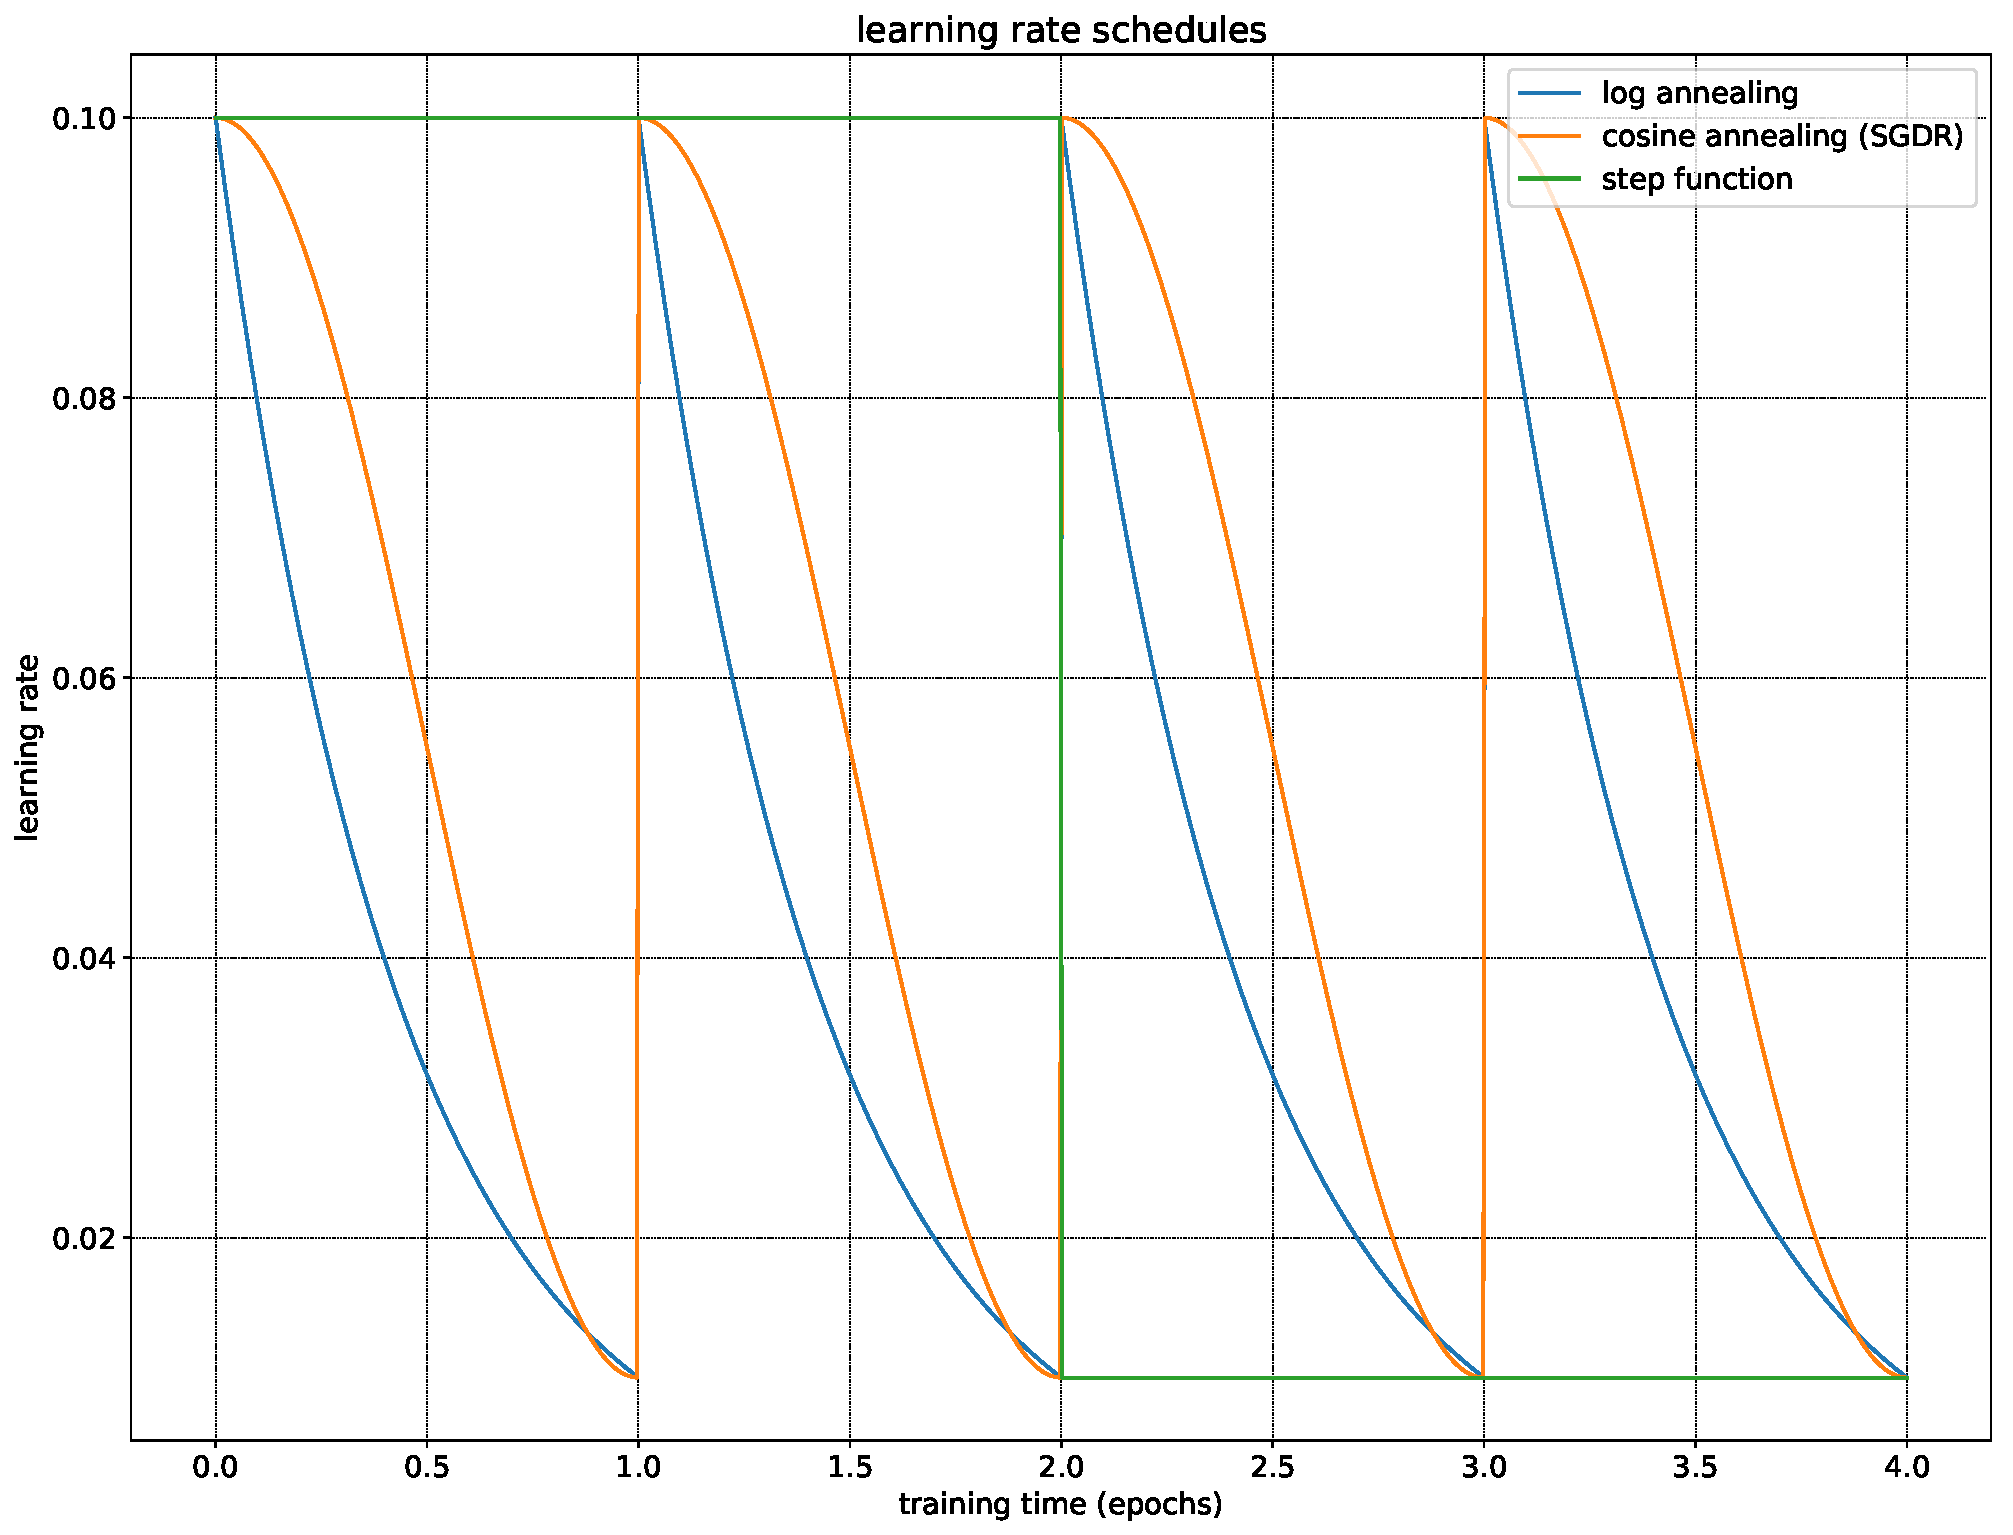
\includegraphics[width=1.0\linewidth]{charts/training/lr_schedules.pdf}
  \caption{Comparison of learning rate schedules, cyclical learning rates and traditional step function.  }  
  \label{fig:lr_schedule}
\end{figure}

In order to facilitate continuous online learning where examples are added over the training lifetime, a cyclical learning rate is used and relatively short learning epochs are used. The idea is that a large learning rate is used for a short period to incorporate information from newly annotated examples, then the learning rate is reduced for a \emph{fine tuning} in order to use the model for inference.

Epochs are set at a fixed size ($1024$ unless otherwise specified), using a uniform random sampling. Learning rates are set for each batch, reducing over an epoch by a factor of $10$, using a logarithmic annealing shown in equation~\ref{eq:log_annealing}. Where $base$ is the base learning rate, and $ t \in [0, 1) $ is the progress across an epoch.

\begin{equation}
annealing_{log}(t) = exp(ln (lr_{min}) (1 - t) + ln(lr_{max})  t)
\label{eq:log_annealing}
\end{equation}

For comparison the learning rate schedule used in \gls{SGDR} \cite{Loshchilov2016}, which has more weight on the highest and lowest learning rates, but otherwise similar.

\begin{equation}
annealing_{cos}(t) = lr_{min} +  \frac{1}{2} (lr_{max} - lr_{min}) (1 + cos (t \pi))
\label{eq:cosine_annealing}
\end{equation}

A comparison of the cyclical learning rates compared to a standard learning rate step schedule is shown for an $8$ epoch training schedule in figure~\ref{fig:lr_schedule}.

\section {Experimental validation}

In this section I evaluate a number of the assumptions which led to the design of the object detector and the annotation tool in general. These hypotheses are:

\begin{itemize}
    \item {It is possible to train object detectors at high resolution using only cropped sections; and keeping images at high resolution will provide more accurate object detection}
    \item {When incrementally adding images through annotation; training the object detector will adapt to new examples better when using a cyclical learning rates}    
    \item {When training a single class object detector it will learn faster than multi-class object detectors}
\end{itemize} 


\subsection {Effect of image resolution and crop size}
\label{sec:scale_crop}


\begin{figure}[h]
  \centering
  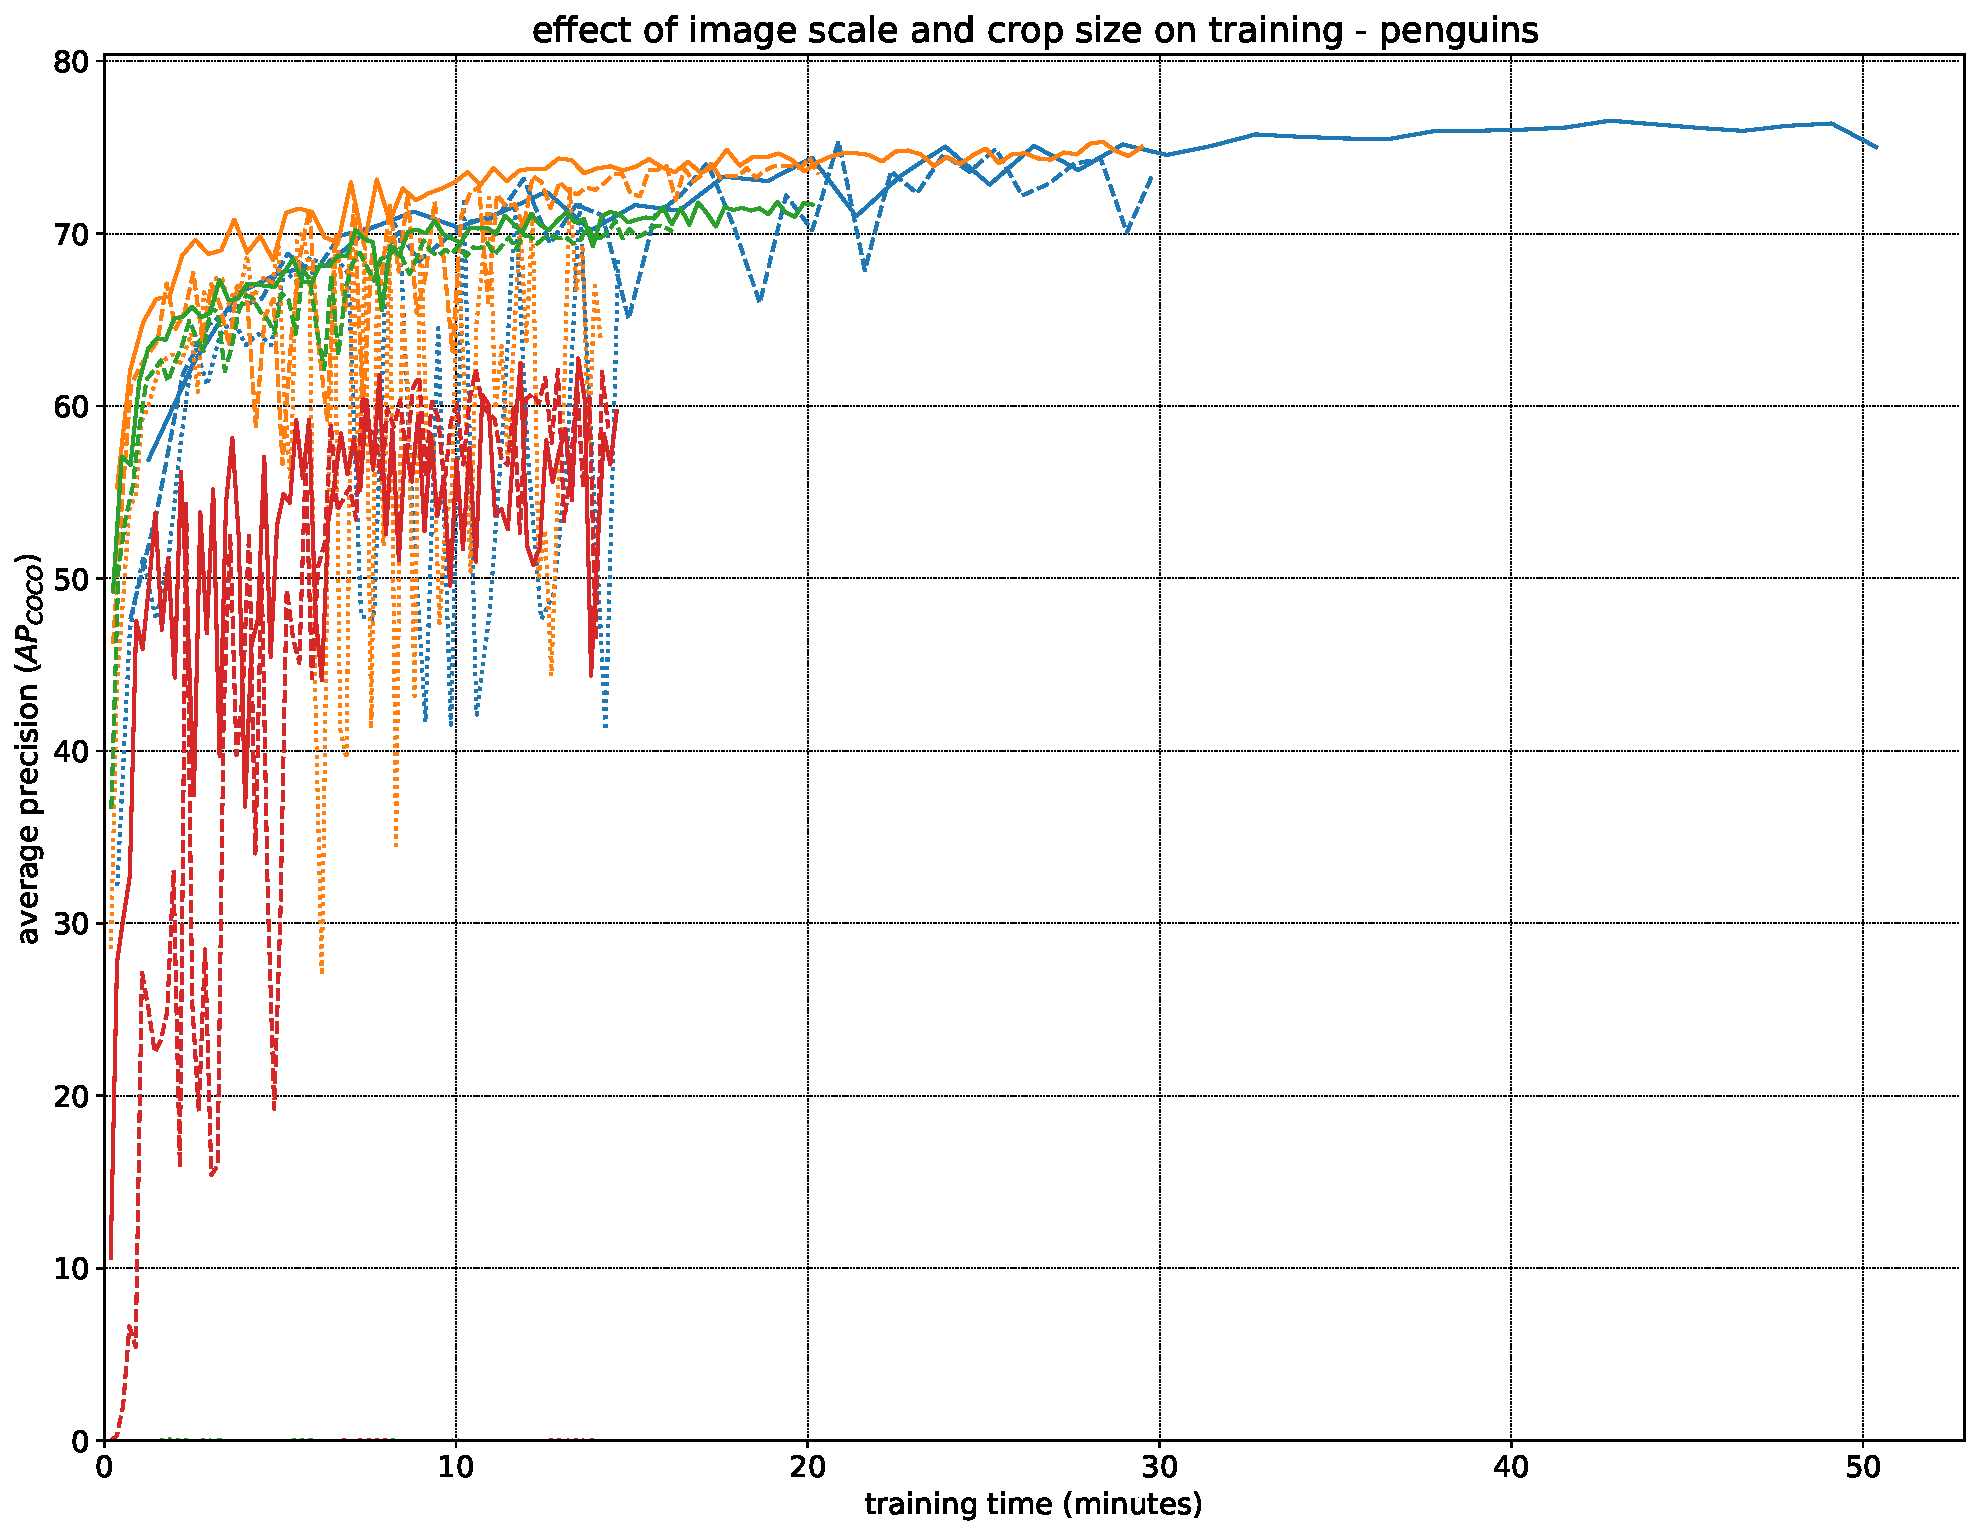
\includegraphics[width=1.0\linewidth]{charts/training/crops_scales/penguins.pdf}
  \caption{Comparison of training at different crop sizes and scales for \emph{apples1} dataset. }  
  \label{fig:apples_crop_scale}
\end{figure}

 
\begin{figure}[h]
  \centering
  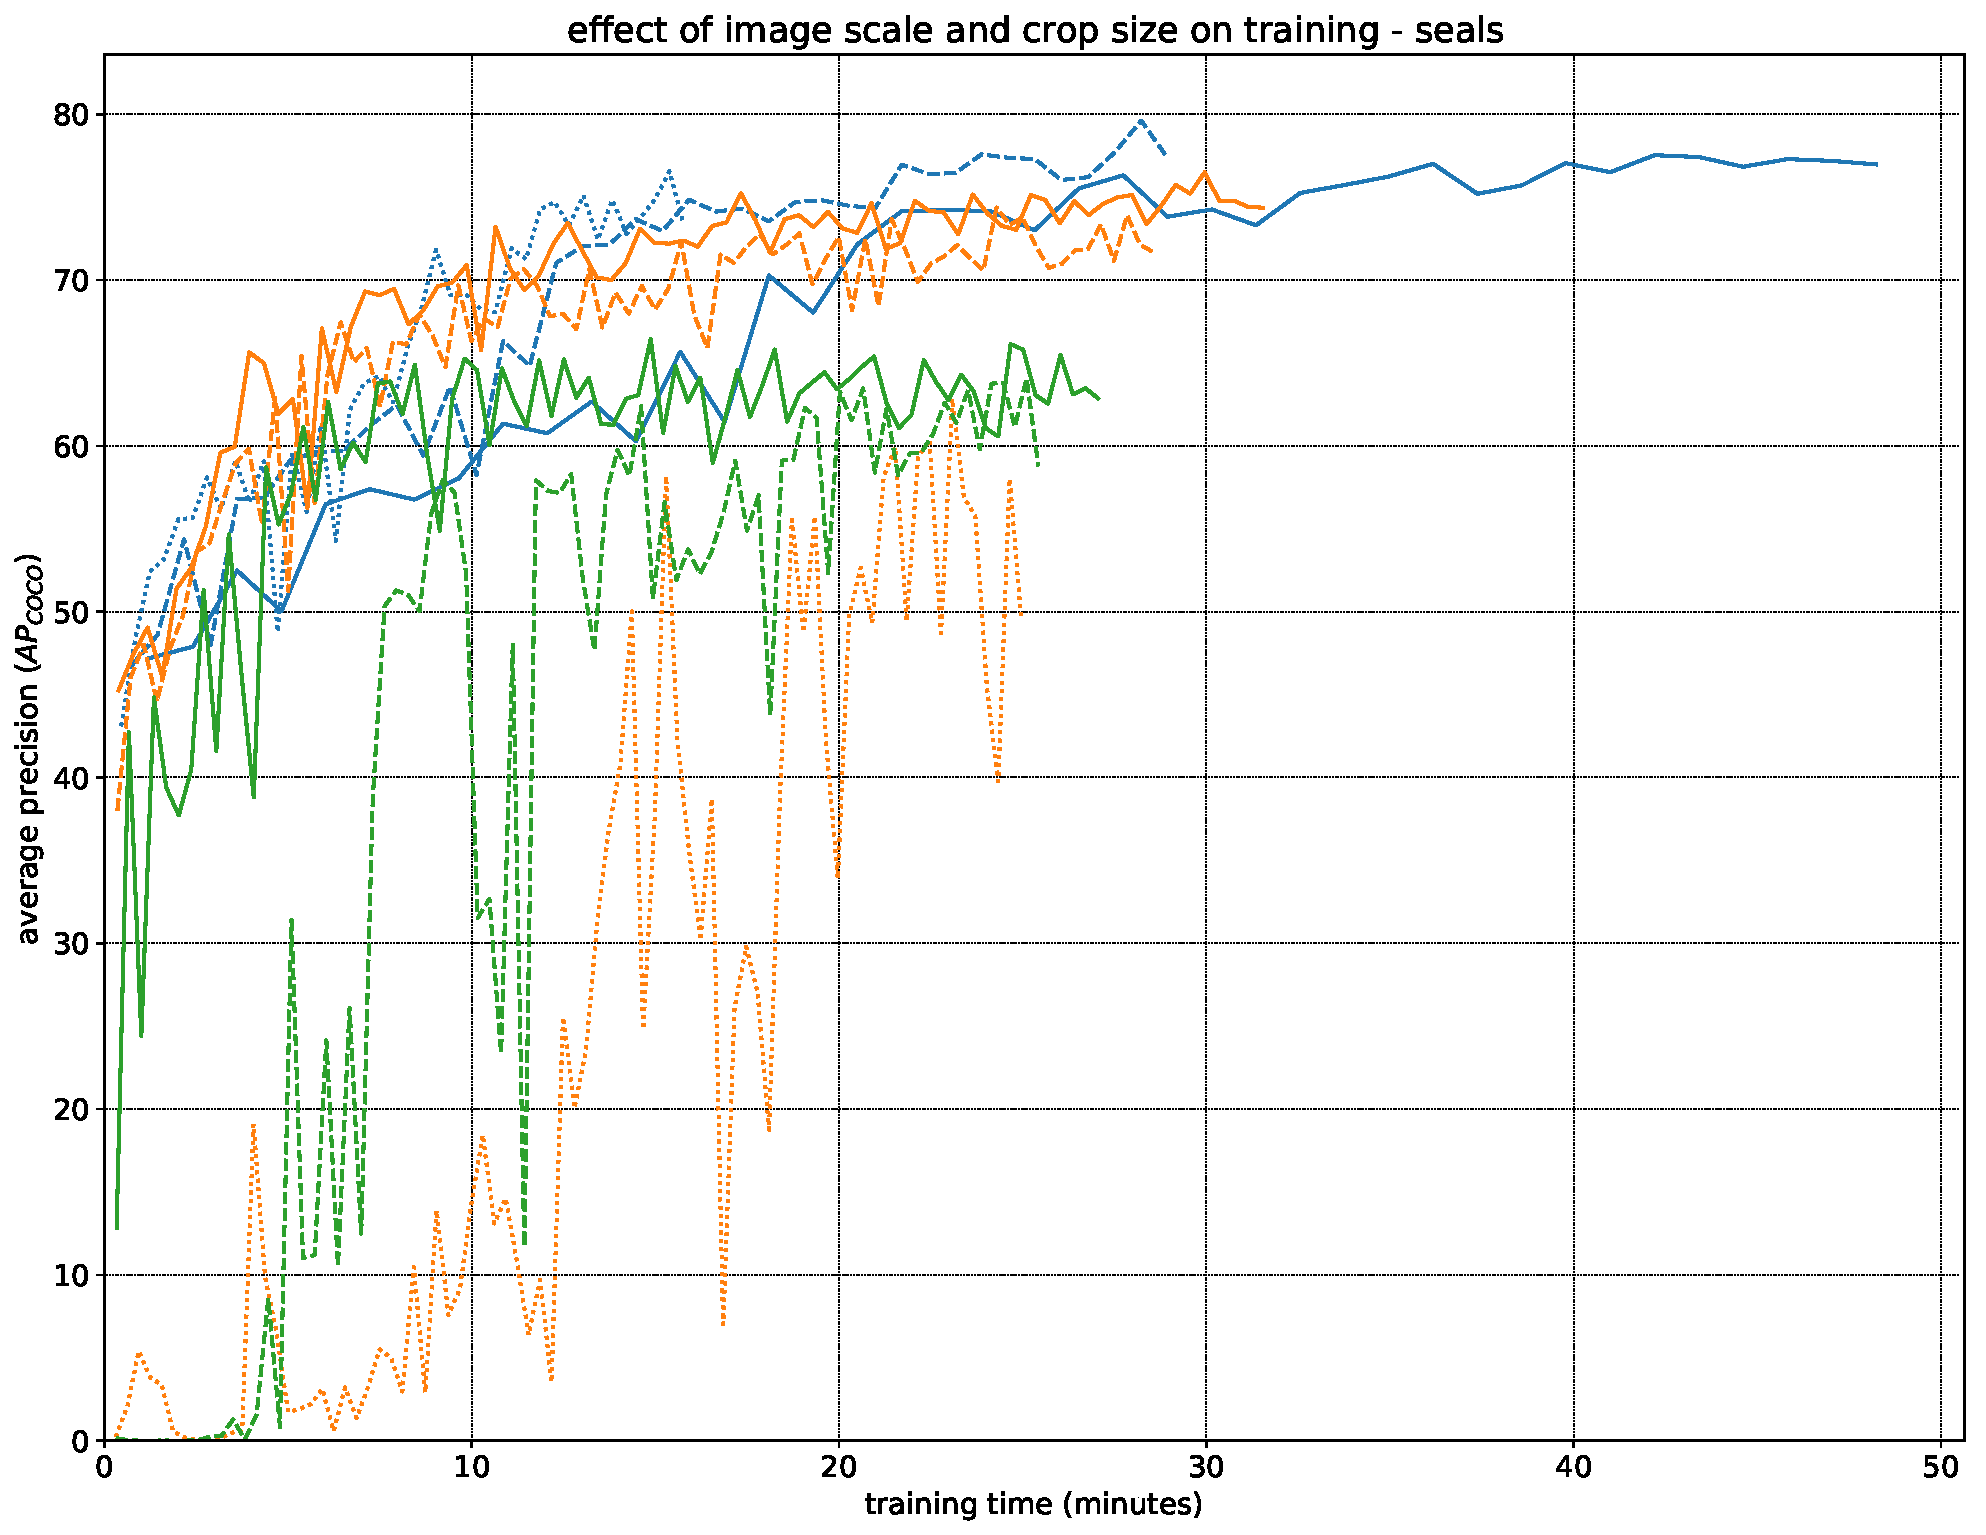
\includegraphics[width=1.0\linewidth]{charts/training/crops_scales/seals.pdf}
  \caption{Comparison of training at different crop sizes and scales for \emph{seals} dataset. }  
  \label{fig:seals_crop_scale}
\end{figure}


\begin{table}[ht]
  \centering
    \caption{Effect of scale and crop size on validation accuracy (percent of best $AP_{COCO}$). Average across datasets (\emph{apples1}, \emph{penguins}, \emph{scallops}, \emph{seals}) }

  \begin{tabular}{ l | l l l l}
    crop/scale & 12.5\% & 25\% & 50\% & 100\% \\
    \toprule
        512   & 0.0  & 2.4  &  59.3  & 82.8 \\
        768   & 17.4 & 68.2  &  90.0 &  96.4 \\
        1024  & 28.5 & 81.9  &  95.0  & 100.0 \\
    \bottomrule
  \end{tabular}
\label{fig:accuracy_scale_crop}
\end{table}


The full resolution provide the best accuracy, although in many of the datasets half resolution provided almost the same accuracy while providing much faster training and inference. At half resolution an ensemble could be trained in similar time to training one network at full resolution and used to provide uncertainty measurements. On the other hand, as seen below in section~\ref{sec:lr_schedule_exp} the training accuracy is limited by the size of the dataset more than the training time, which is severely dependent on human annotation time which will allow plenty of time for training at high resolution.

The training speedup is measured, note the figure for training time is just the training time, and excludes time for validation. It would be expected that halving image resolution would halve the training time, but that figure is instead around $3.3$ (and for lower resolutions much higher). The reason for that is that the images are still being loaded at full resolution, so the bottleneck becomes the image loading.

\begin{table}[ht]
  \centering
    \caption{Speedup associated with reduced resolution. Average across datasets (\emph{apples}, \emph{penguins}, \emph{scallops}, \emph{seals})  }
  \begin{tabular}{ l | l l l l}
    crop/scale & 12.5\% & 25\% & 50\% & 100\% \\
    \toprule
        512   & 6.0  & 5.9  &  5.9  & 3.3 \\
        768   & 5.9 & 5.3  &  4.4 &  1.7 \\
        1024  & 5.9 & 4.5  &  3.3  & 1.0 \\
    \bottomrule
  \end{tabular}
\label{fig:accuracy_scale_crop}
\end{table}


Using a larger crop size proved more accurate in all of the four datasets, and using a larger crop was beneficial in all cases, being more accurate and more stable to train. The larger size however trains much more slowly, so in an active learning system it is possible to use the time savings for other things such as evaluating unseen images for the purposes of example selection; or training a set of several models to use as an ensemble.


\subsection {Inference method for large images}

\begin{figure}[h]
  \centering
  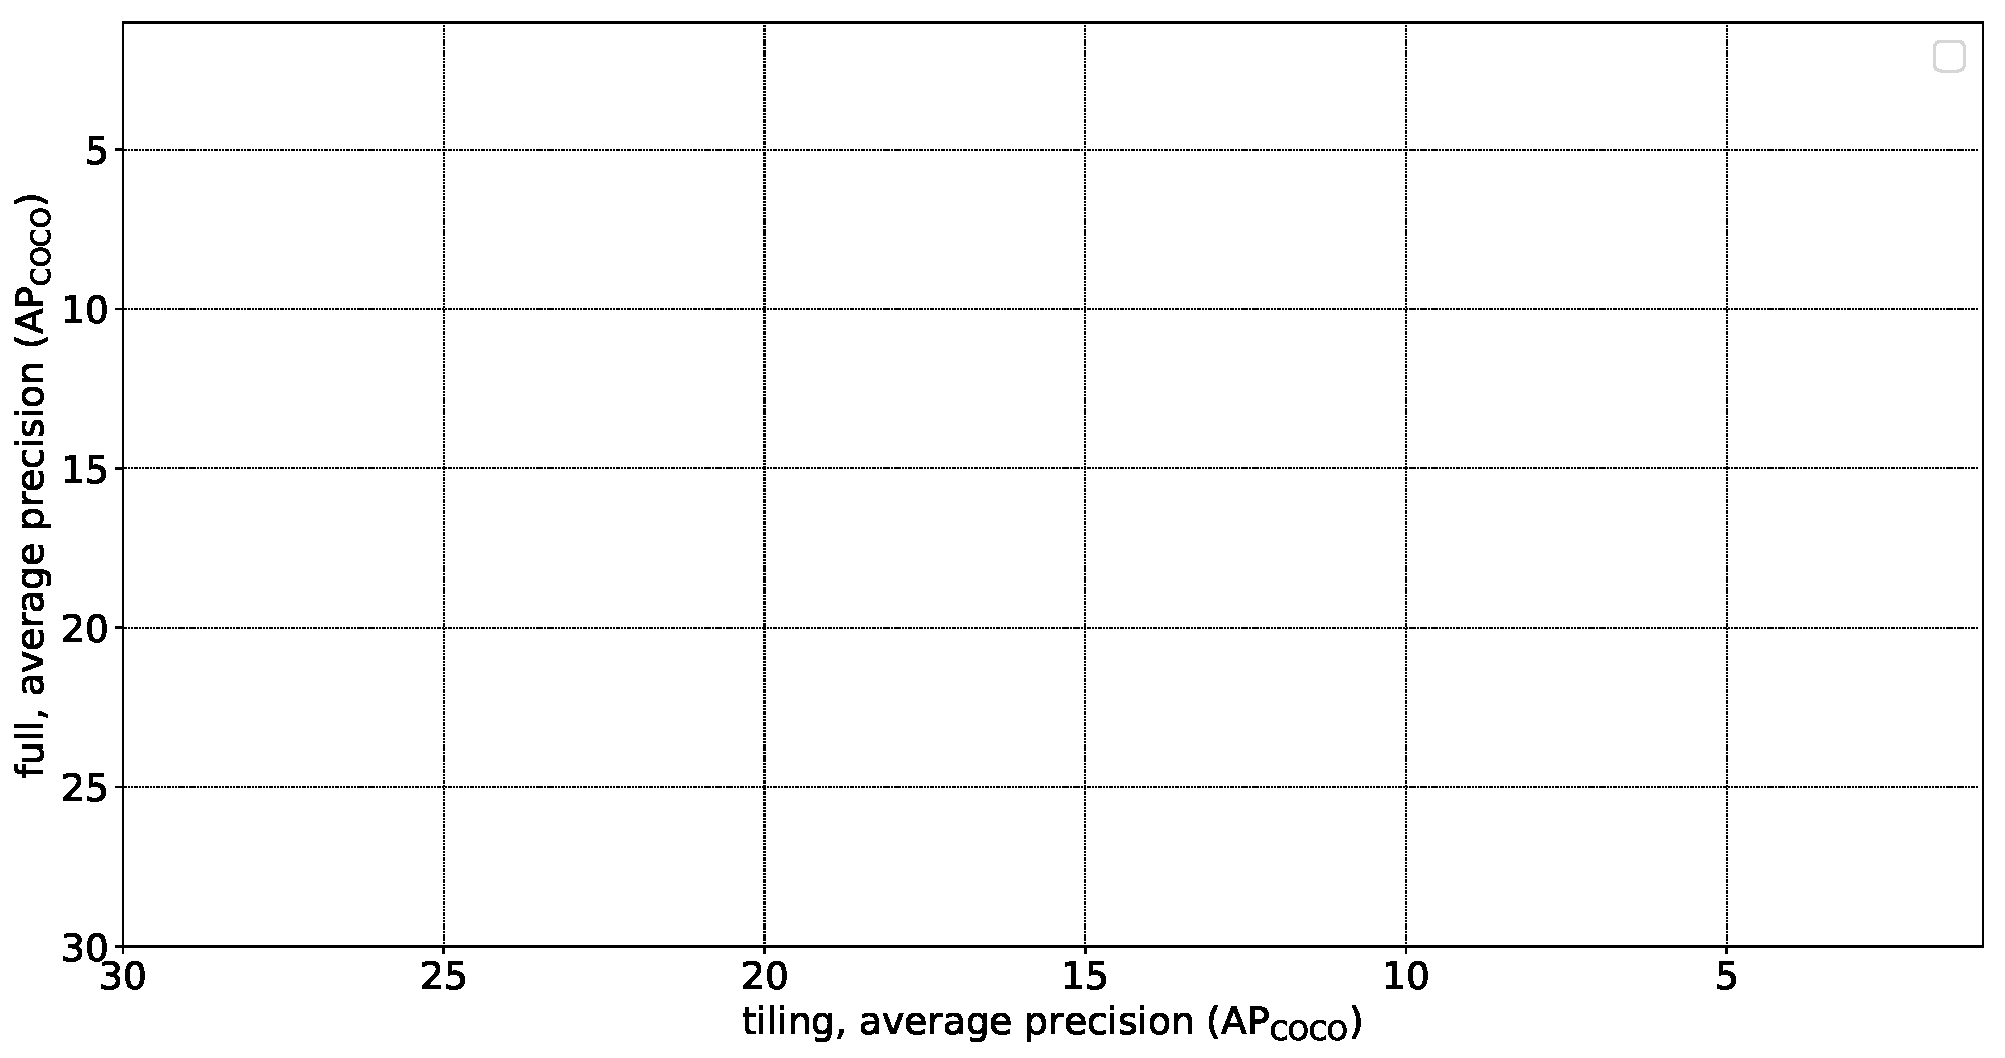
\includegraphics[width=1.0\linewidth]{charts/training/splits_scatters.pdf}
  \caption{Comparison of different inference methods across one training run, inference using tiling vs. inference on full images. Training occurs on crops and evaluating on full images. }  
  \label{fig:inference_method}
\end{figure}


I compared the two methods (tiling vs. inference on the full image) by using both methods for testing against the validation set of several different training runs. It can be seen in figure-\ref{fig:inference_method} that both perform very similarly. If there is ever a difference; sometimes one is marginally better, sometimes the other is marginally better, even within the same training run.


\subsection {Learning rate scheduling}
\label{sec:lr_schedule_exp}

In this work I use cyclical learning rates, with the aim of adjusting faster to stream of new examples (as occurs during an annotation process), this is important if the model is to provide good assistance to an annotator in a timely fashion. Here I aim to test this assumption, which is done by training a set of datasets with a variety of learning rate scheduling settings. 

I test in two settings, \emph{full}: where the entire training set is available from the beginning of training; and \emph{incremental}: where only a subset of the training set is used for training. The size of that subset used being a fraction of the full training set where the fraction used is the progress through training; so, for example in a training run of $40$ epochs, half way through (after $20$ epochs) $50\%$ images are used for training. 

The tests include using longer (4096 images per epoch) and shorter (1024 images, as used in the rest of this work) learning rate cycles, using log annealing and cosine annealing and comparing against a baseline where the learning rate is the step function, half way through training is reduced by a factor of $10$.

\begin{figure}[h]
  \centering
  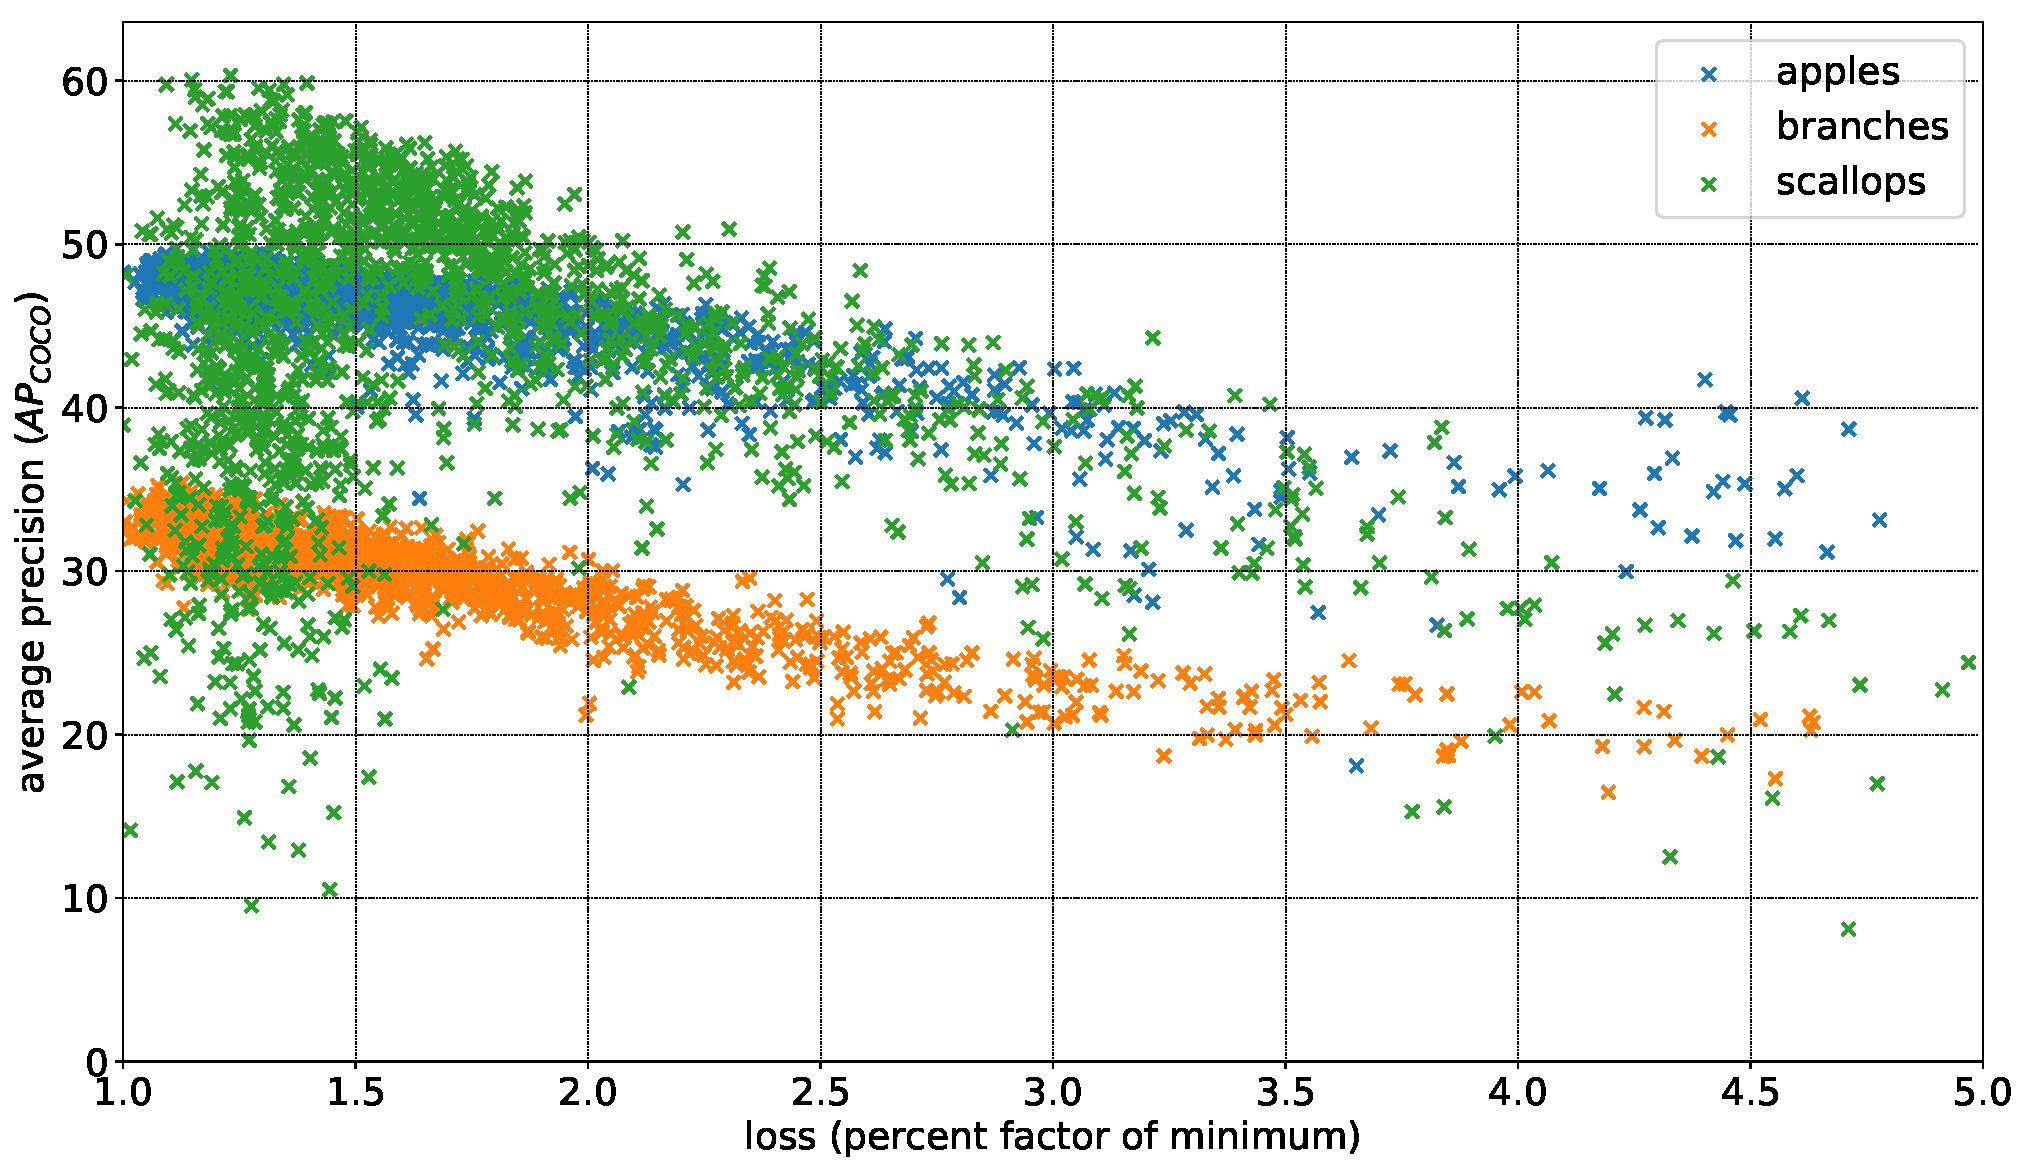
\includegraphics[width=1.0\linewidth]{charts/training/lr_schedule/scatter_loss_ap.pdf}
  \caption{Correlation between loss function and validation $AP_{COCO}$ for three different datasets across 6 repeated training runs (non incremental case)}  \label{fig:scatter_loss_ap}
\end{figure}

The tests showed a considerable amount of noise, especially for the \emph{scallop} dataset, so it was repeated 6 times to attempt to distil anything useful from it. Figure~\ref{fig:scatter_loss_ap} shows the differences in variability between the three datasets used, the \emph{scallop} case, in particular the correlation between low loss and high validation \gls{AP} is noisy, and in the \emph{scallop} case extremely noisy. 

\begin{figure}[h]
  \centering
  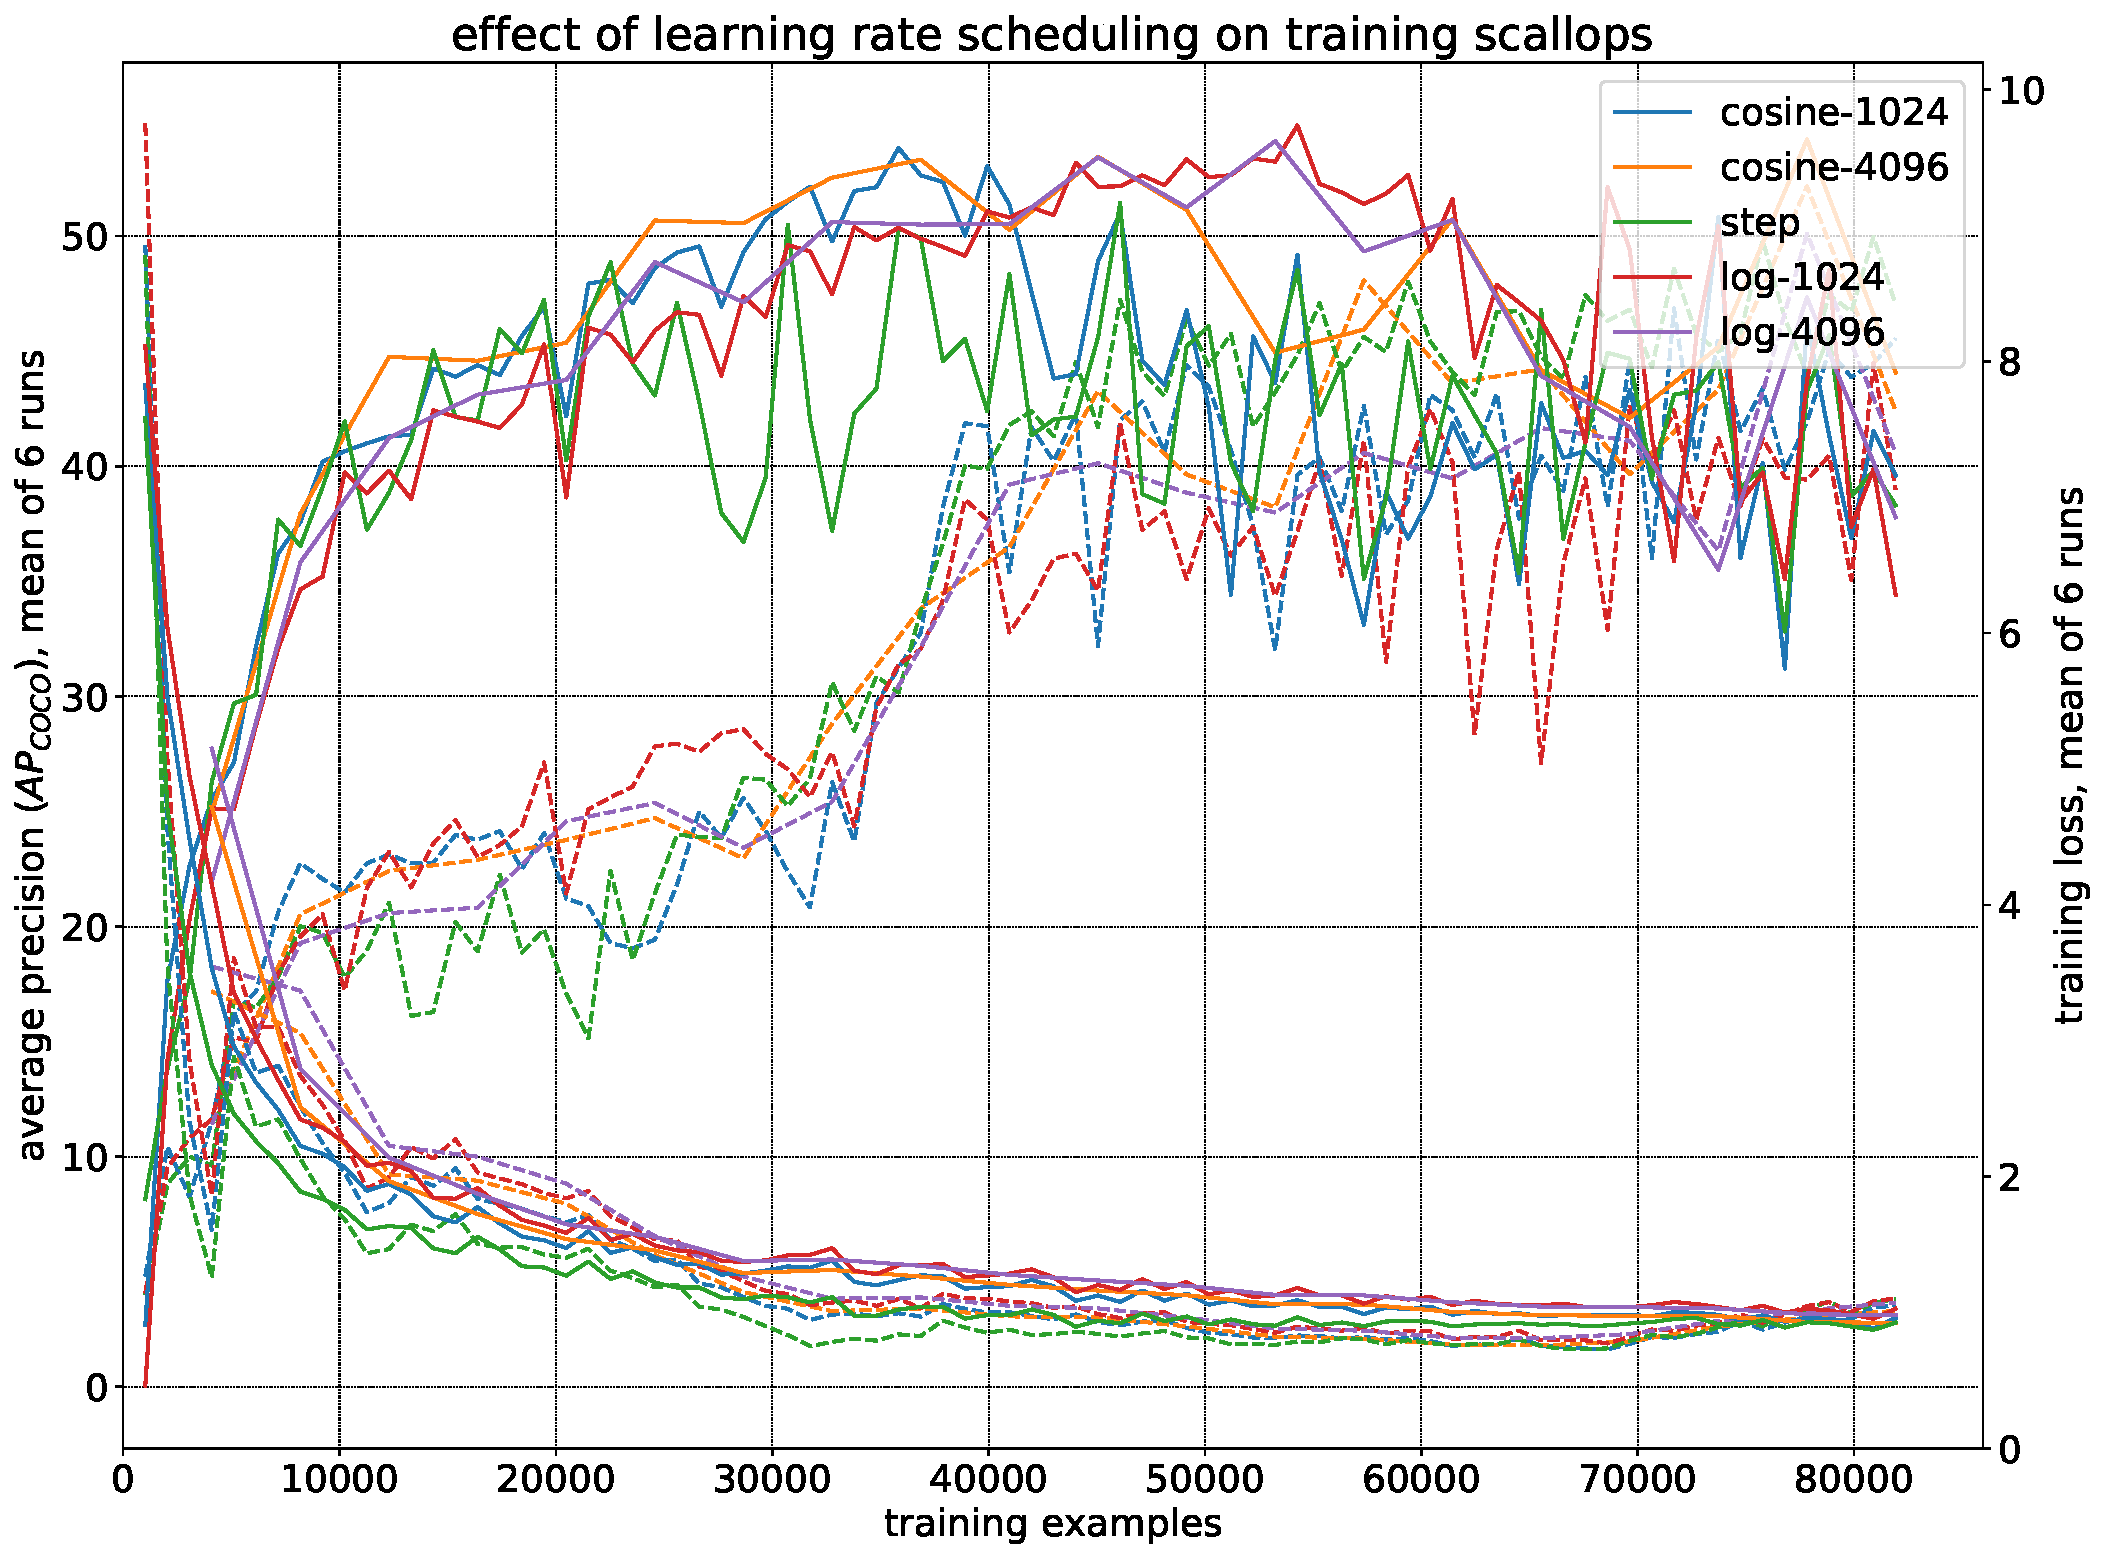
\includegraphics[width=1.0\linewidth]{charts/training/lr_schedule/scallops.pdf}
  \caption{Training of the \emph{scallop} dataset, the bottom lines show the loss function and the top show validation $AP_{COCO}$}  
  \label{fig:scallop_lr}
\end{figure}

\begin{figure}[h]
  \centering
  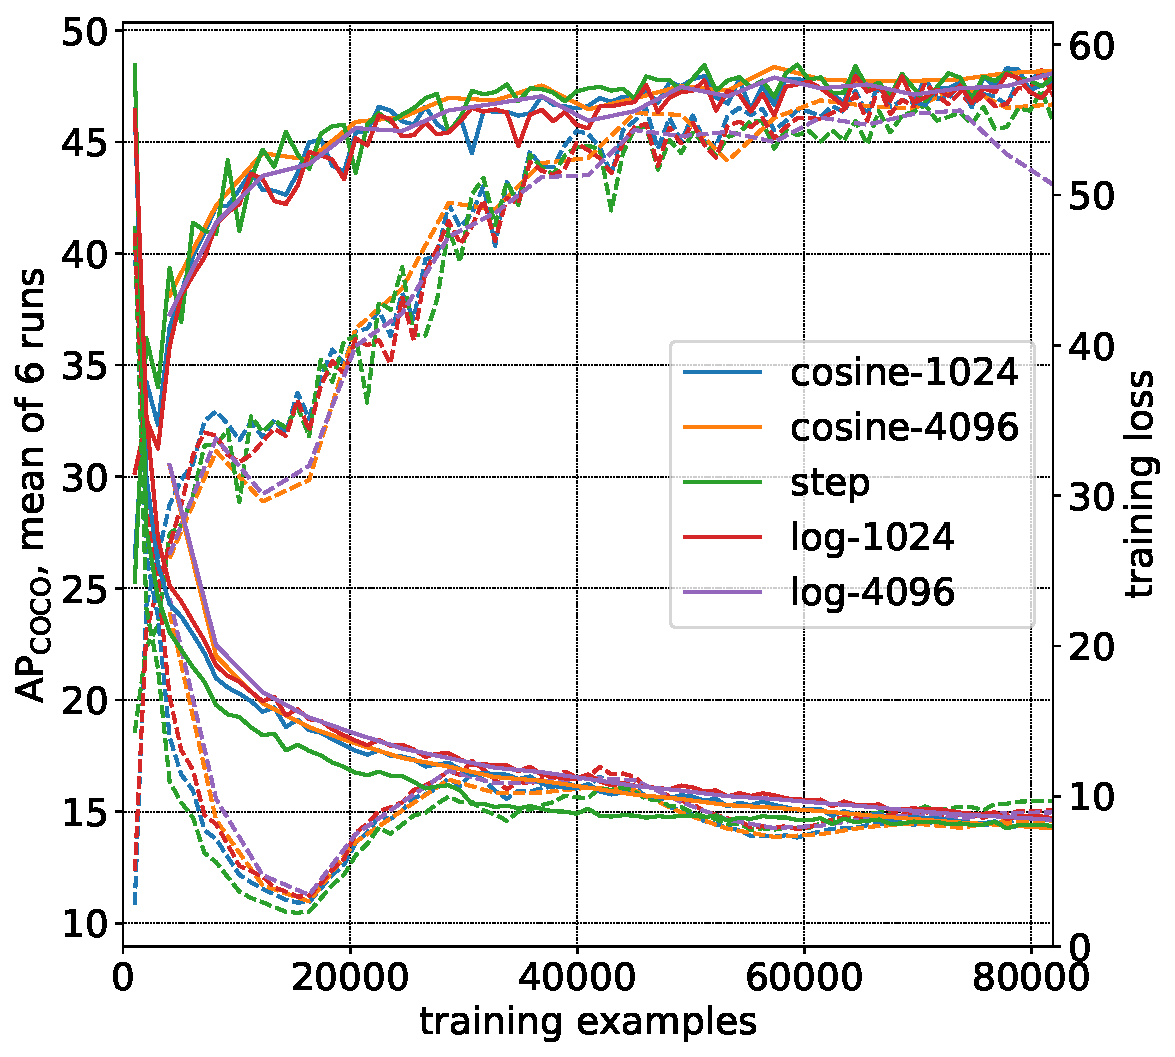
\includegraphics[width=1.0\linewidth]{charts/training/lr_schedule/apples.pdf}
  \caption{Training of the \emph{apples1} dataset, the bottom lines show the loss function and the top show validation $AP_{COCO}$}  
  \label{fig:apple_lr}
\end{figure}

Figures~\ref{fig:apple_lr} and \ref{fig:scallop_lr} show training runs for \emph{apples1} and \emph{scallop} datasets, the pattern for \emph{branches} was very similar to \emph{apples1}. A noticeable pattern can be seen in the incremental case where the validation \gls{AP} increases positively with the number of examples used in training, showing that the factor limiting the accuracy is the size of the dataset (the number of annotated images so far).

There seems little differences of note between learning rate schedules in terms of either the validation accuracy or the amount the loss is reduced. At the beginning the \emph{incremental} loss is reduced much faster than the \emph{full} case, because it is able to fit the small number of examples much better. The constant learning rate reduces the loss better in the early part of training, but towards the end there seems little difference between the different methods. 

Further study will be required on larger datasets to determine if this is something useful to persevere with, on this small experiment alone there seems using the cyclical learning rate is much less important than was expected.

\subsection{Single or few-class vs. multi-class}
\label{sec:multiclass}

\begin{figure}[h]
  \centering
  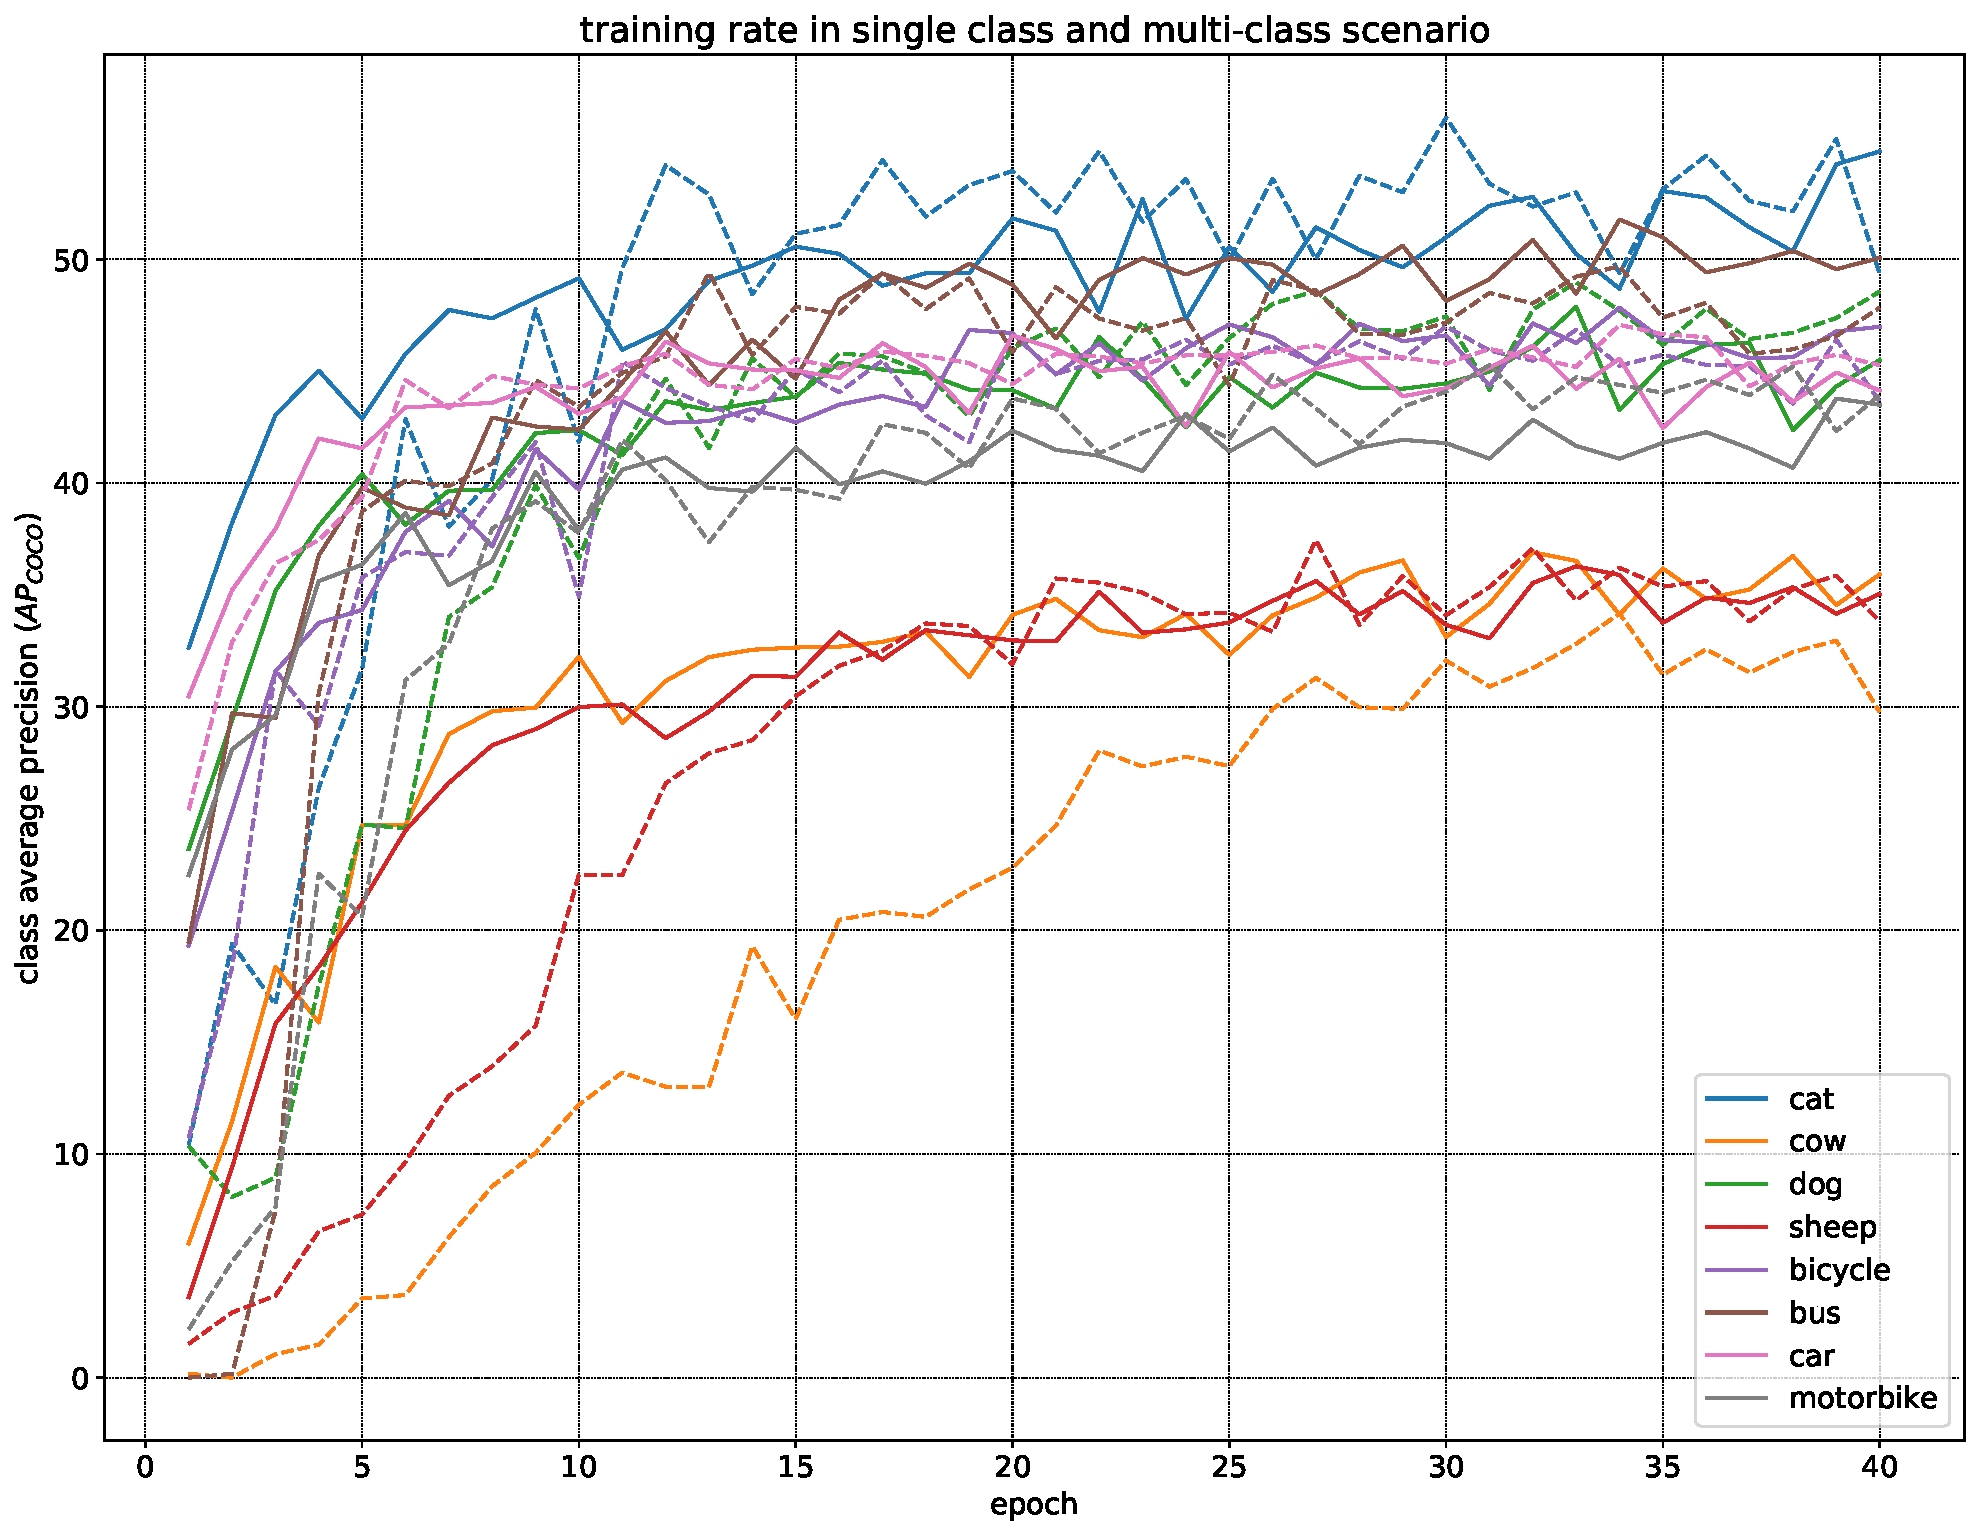
\includegraphics[width=1.0\linewidth]{charts/training/multiclass.pdf}
  \caption{Single class vs. multi class for selected classes of the Pascal VOC dataset. Dotted lines are test $AP_{COCO}$ for classes trained 4 at a time; solid lines are trained a single class at a time. }  
  \label{fig:multiclass}
\end{figure}

In this experiment I test the hypothesis that an object detector trained with single-class training learns faster than multi-class training. For this the Pascal VOC \cite{Everingham2008} dataset is used. Training is performed on the train 2012, train 2007 and validation 2012 subsets, and tested on the 2007 test set.I use two subsets of images comprising each comprising of a set of images containing any object in set of four classes. First an object detector is trained in the multi-class scenario on all four classes, afterwards each of the four classes is trained individually. 

The network feature sizes were not adjusted between single-class and multi-class scenarios, so the network is learning more in the same sized features and number of parameters. It has been seen that in practice larger networks and over-parameterisation generalise better to a range of image datasets \cite{Kawaguchi2017}, although supported more weakly by theory so far \cite{Du2018a,Lee2019}. In using single-class training, but using network capable of detecting many classes, the parameterisation is much larger compared to a multi-class setting. In this work a relatively simple model is used, ResNet-18, but such a model is also capable of classifying ImageNet to reasonable accuracy with $1000$ classes.

For practical inference training a single model which detects objects of many classes (as opposed to many single class models) at once presents obvious benefits but for annotation; such as synergy of feature representations and computational efficiency. If we can get away with learning for as few classes as is practical there may be some benefit. 

  Note that in each instance the set of images is the same, so in the single class setting a large portion of the images will essentially be negative images. In a real annotation scenario the negative images can be sampled less often, or a larger quantity of images of the same class can be annotated first.

The resolution used is 512 pixels, trained with the same training method, image preparation etc. as other experiments in this chapter. The learning rate used was 0.01 (higher than other experiments) as it learned faster on the VOC images, a batch size of 16 and epoch size of 8192 was used, and the models trained for 40 epochs (comparatively much longer than the annotated datasets used in this thesis).  

The results can be seen in figure~\ref{fig:multiclass}. It shows that although both multi-class and single-class accuracy eventually reached approximately the same level; the single-class accuracy was reached faster in all cases, and in a few cases much faster (especially the \emph{sheep} and \emph{cow} classes). This experiment shows that in this somewhat limited setting at least, the single-class training is faster.



\section {Conclusion}

This chapter described the object detector used behind the annotation tool, parameters used, methods of training and described some of the rationale for the differences with published literature. I performed some experiments to attempt to validate some of the ideas used in the design of the object detector (for the purposes of use in a verification based annotation tool). 

I show that the high resolution approach; by training with image crops provides higher accuracy for the datasets tested at the expense of training efficiency. In each case using larger crop sizes proved better, with smaller crop sizes being less accurate and destabilising training. Two different methods of inference at high resolution were tested, one by using the property of the \gls{FCN}, the other by tiling---both were found to be approximately equal, with one trading off time, the other memory usage.

Training with cyclical learning rates was shown to perhaps be less important than assumed; at least in the experimental conditions used here. There existed little difference between training with constant learning rate and the various forms of cyclical learning rate. Testing with incrementally adding training images showed the generalisation was limited by the number of examples added.

I investigated if training single classes (as well as annotating single classes) was faster in a small trial using the Pascal VOC dataset. In these conditions, training on a single class performed better much sooner in training in each case.



